\section{Literature Review}
\label{sec:literature}
The advent of modern object detection has enabled more sophisticated and automated methods for understanding visitor engagement and flow in cultural institutions. This literature review aims to explore the current state of research on the various topics of this thesis. This includes visitor behaviour analysis and stakeholders perspectives, individual privacy, object detection, the influence of fine-tuning models on specialized data, and existing third-party services for deploying similar person localization systems.

\subsection{Visitor Behaviour Analysis and Stakeholder Perspectives}
\label{sec:visitor_behaviuor_analysis}
Some of the traditional methods of analyzing visitor behaviour include surveys, manual counting, and direct observation. Today, more technology-driven and practical applications may be used to gain insights in visitor engagement and experience in a museum or aquarium setting. In this subsection, we look at an alternative to computer vision tracking systems. Afterwards, a study on the perceived value of visitor tracking to museum stakeholders is brought foreward.

\subsubsection{Questions Asked by Visitors in a Mobile App}
\citeauthor{co2023appquestionairre} had visitors ask questions in a mobile app while moving through the museum \citeyear{co2023appquestionairre}. Visitor movement through the museum was inferred from the data by leveraging question keyword content, knowledge of exhibit layout, and question timestamps. This removed the need for more costly, vision-based applications for detecting and tracking visitor movement. This study illustrates one way of conducting affordable, dependable and scalable visitor analysis without the need for costly devices.

\subsubsection{Perceived Value to Museum Stakeholders}
\citeauthor{la2017museumbehaviouranalysis} explored an alternative approach to museum visitor behaviour analysis, and its perceived value to museum curators, administrators and department heads (\citeyear{la2017museumbehaviouranalysis}). Wearable RFID trackers\footnote{The requirement for visitors to wear RFID trackers represents a significant drawback as it may be perceived as intrusive (although completely privacy preservant).} were given to the visitors, and beacons were positioned at positions deemed important by the museum curators. The beacons would then communicate the positions of the visitors to the system. This allowed for the collection of data on key metrics like exhibit popularity, average visit duration, and common visitor paths. The authors noted that technology-based visitor behaviour analysis was generally well-received by museum curators, offering valuable data that could enhance the visitor experience.

The study of \citeauthor{la2017museumbehaviouranalysis} further discussed the divergent views between the curators and the administrators on the utility of visitor behaviour analysis systems (\citeyear{la2017museumbehaviouranalysis}). Administrators and department heads generally viewed these systems favorably, citing the financial justification for expensive exhibitions: \textit{We really need to know if this expenditure was worthwhile} (\cite{la2017museumbehaviouranalysis}). On the contrary, museum curators expressed skepticism. One curator remarked: 

\begin{myquote}
    A temporary exhibition won't change after you deploy it, and understanding how it is used by the public would not help me in my next exhibition, since they are each very different. My main reason to analyze behaviour would be to satisfy my curiosity. (\cite{la2017museumbehaviouranalysis})
\end{myquote}

This contrast underscores the varied perspectives within museums regarding the value and implications of behaviour analysis technologies. 

\subsubsection{User Perceptions of Smart Home Privacy}
\label{sec:smarthomeprivacy}
In a 2018 study, researchers conducted semi-structured interviews of 11 smart home owners were conducted to figure out user perceptions of smart home IoT privacy and obsoleteness as there are frequent upgrades and new products on the market (\cite{zh2018userperceptionsofIoTPrivacy}). Responses regarding the privacy demands versus an increase in convenience of the IoT devices were concerning:

\begin{myquote}
    I think it's more likely that a lot of these things will become obsolete... If that's what happens then I have to buy another device. It still might be worth it for the convenience. (Participant 10)
\end{myquote}

\begin{myquote}
    [The security concern] is always kind of in the back of my mind because of all that IoT stuff that always goes on, and everyone says how easily hackable they are. But I think my peace of mind that I get from having them outweighs my worry of what could be potentially taken advantage of. (Participant 6)
\end{myquote}

These responses indicate that the convenience and connectedness of the devices surpass the desire to preserve privacy\footnote{Connectedness of IoT is still an issue since there is no standard communication protocols. Matter is a Zigbee-based wireless protocol that operate as an application layer on top of Thread, Ethernet or Wifi. It allows IoT devices to communicate, but it is not yet widely adopted. This may be due to the high costs, as the Connectivity Standard Alliance demands a yearly membership for the rights to use th CSA's trademarks. Additionally, the devices must be certified for security, adding extra costs as many companies must buy this certification service. Another great improvement in terms of connectivity that does not limit privacy is the EU regulation that all smaller devices sold after 2024 must have USB-C connection. This also applies to laptops in 2026.}. This is a promising finding for the development of visual systems in museums and aquariums, as it suggests that the benefits of the system may outweigh the privacy concerns of the visitors. It also illustrates the need for regulations to prevent solutions from being developed that are too privacy-invasive, as the end-users will not prioritize privacy over convenience.

\subsection{The General Data Protection Regulation (GDPR)}
\label{sec:GDPR}
The general data protection regulation (GDPR) is a single set of regulations to guarantee privacy and protection of personal data. A quick review of the GDPR should be on the agenda of anyone affiliated with systems not inherently preservant of privacy\footnote{More specifically, \textit{informational} privacy. This term is introduced in \ref{sec:individual_privacy}}.

The GDPR entered into applicability in the EU on 25th of May 2018 has two major impacts. 1) It leaves individuals with more control over their data, and 2) it facilitates a level playing field for all companies; there is now a single set of data protection rules for all companies operating in the European Economic Area (EEA)\footnote{The EEA consists of all EU countries plus Iceland, Liechtenstein and Norway.}. The most relevant sections of the GDPR to this thesis are the regulations regarding personal data.

\subsection{Personal Data}
\phantomsection
\label{sec:personal_data}
Personal data is any form of information that can be connected to an identifiable data subject. The following definition was given by the european parliament in 2016:

\begin{myquote}
    The term 'personal data' means any information relating to an identifed or identifable natural person ('data subject'); an identifable natural person is one who can be identifed, directly or indirectly, in particular by reference to an identifer such as a name, an identifcation number, location data, an online identifer or to one or more factors specifc to the physical, physiological, genetic, mental, economic, cultural or social identity of that natural person. (\cite{in2023gdpr_website})
\end{myquote}

Privacy, which is closely knit to personal data, is more discussed in Section \ref{sec:individual_privacy}. First, we take a look at some approaches to managing personal data. 

\newpage
\paragraph{Approaches to Managing Personal Data}
Various methodologies can be adopted to manage personal data within a system. 

One approach involves transforming information so that it no longer qualifies as personal data. This can be achieved through techniques such as differential privacy, which ensures that the processed data cannot be traced back to an individual. See Section \ref{sec:differential-privacy} for a detailed explanation of differential privacy. 

A second approach for managing personal data involves establishing lawful grounds for the processing of personal data. This necessitates adherence to legal frameworks that justify the use of personal data under specified conditions, thereby ensuring compliance with data protection regulations. Processing of personal data is permissible under the GDPR only when it satisfies at least one of the following legal bases:

\paragraph{Legal Bases for Processing Personal Data}
\label{sec:legal-bases-processing-personal-data}
\begin{itemize}
    \item The data subject has given explicit consent.
    \item It is necessary for the performance of a contract to which the data subject is a party.
    \item It is necessary for compliance with a legal obligation to which the controller\footnote{The controller refers to the party controlling the data} is subject.
    \item It is necessary to protect the vital interests of the data subject or of another natural person.
    \item It is necessary for the performance of a task carried out in the public interest or in the exercise of official authority vested in the controller.
    \item It is necessary for the purposes of the legitimate interests pursued by the controller or by a third party, except where such interests are overridden by the interests or fundamental rights and freedoms of the data subject which require protection of personal data.
\end{itemize}

Additionally, the controller is responsible for compliance with the 3 requirements summarized below and should be able to demonstrate this compliance at any given time.

\begin{itemize}
    \item{Security Documentation}
    In the event of a breach of personal data, the controller must document that proper precautions were made to secure the data. One of these precautions is to deleted data that is no longer needed. This rule to delete no-longer-needed data is often overlooked and violated by companies (\cite{sa2022webinar_gdpr}).
    \item{Data breaches}
    Breaches of personal data must be reported within 72 hours. Companies failing to do so are economically sanctioned, but even worse, it damages the reputation of the company. In such cases it is common to uncover more failures (\cite{sa2022webinar_gdpr}). This is often that the company has failed to make, or failed to document, the efforts they have made to sufficiently protect the data (the first requirement).
    \item{Rights of the data subject}
    The data subject has the right to be informed about how their personal data is handled. This is commonly achieved through the company's privacy declaration, which must be comprehensive and regularly updated. Additionally, companies are encouraged to proactively communicate this information to clients, for instance, via email. According to privacy experts (\cite{sa2022webinar_gdpr}), adopting such practices is an effective way of building and maintaining trust with customers.
\end{itemize}
    
There are multiple other approaches for managing personal data that are more specific to the management of \textit{images}. The ones discussed in this thesis are primarily concerned with removing the individual information of persons from the images. These methods are discussed in Section \ref{sec:individual_privacy}. 

\subsection{The Network \& Information Security 2 (NIS2) Directive}
\label{sec:NIS2_relevance}
    
The NIS2 Directive (\cite{eu2022nis2}) is a more recent EU regulation that came into force in January 2023. Unlike the GDPR, which broadly addresses the protection of personal data, NIS2 is specifically targeted toward technology. As an update to the EU's cybersecurity framework, NIS2 focuses on strengthening the security of network and information systems. It emphasizes the critical need for robust security measures in systems that process personal data to prevent unauthorized access and data leaks.

Both NIS2 and GDPR highlight the principle of data minimization, which mandates that object detection systems process only the necessary amount of personal data for their intended function. This practice not only bolsters security but also supports privacy by minimizing potential data exposure. Adhering to these principles is vital for maintaining user trust and ensuring compliance with EU regulations, particularly when deploying object detection technologies in environments where data sensitivity is paramount.

\subsection{Preservation of Individual Privacy in Images}
\label{sec:individual_privacy}
Building on the previously introduced regulations in Section \ref{sec:GDPR}, the contents of this section aims to provice a deeper insight into the methods of preserving the individual privacy of individuals \textit{in images}. It is heavily influenced by previous work of the same author. See the disclaimers in Section \ref{sec:disclaimers} for more details.

The first definition of privacy was given by \citeauthor{br1890righttoprivacy} in \citeyear{br1890righttoprivacy} as \textit{the right to be let alone}. A more comprehensive definition of privacy that is more relevant to the modern age of digitalization and the topics of this thesis is the following:

Privacy as informational self-determination:

\begin{myquote}
    Privacy is the claim of individuals, groups and institutions to determine for themselves, when, how and to what extent information about them is communicated to others. (\cite{we1967privacydefinition})
\end{myquote}

There are multiple dimensions to privacy. The definition of \citeauthor{we1967privacydefinition} covers informational privacy, which is most relevant to this thesis. This definition includes groups and institutions, however, in most legal systems, privacy is defined as a basic human right that only applies to natural persons\footnote{A natural person (also sometimes referred to as a physical person) is a title used to identify an individual human being. This is different from a legal person, which can be an individual or a company (\cite{te2023naturalperson}).}. The term \textit{individual privacy}\footnote{Individual privacy is sometimes referred to as personal privacy.} encapsulates the individual focus of privacy as opposed to the broader interpretations of privacy that might apply to groups, organizations, or institutions. Other dimensions of privacy include spatial privacy, territorial privacy, and bodily privacy (\cite{fi2017privacybookchapter53}). These will not be further discuss in this thesis.

Preservation of individual privacy refers to maintaining the personal space and confidentiality of individuals, ensuring that their private lives and personal integrity are not invaded or exposed (without consent). 

Protection of personal data is important due to the regulations, preserving the individual privacy is also essential to maintain trust with customers, and to avoid (\textit{delay}\footnote{See Section \ref{sec:discussion_ethics_localization_tech}} for brief discussion on the ethicality of person localization systems development.) the onset of a dystopian society...

\newpage
\subsubsection{Privacy in Images}
\label{sec:preservation_individual_privacy_in_images}
Protection of personal data in general is very similar to protection of personal data in images. Protection deals with the management and security of personal information—data that can identify an individual, such as names, addresses, and biometrics. This protection is primarily about the correct handling, processing, storage, and destruction of personal data to prevent unauthorized access, misuse, or breaches. 

There are multiple methods, both pre- and post-processing, for preserving individual privacy in images. One example of a pre-processing privacy preservation method is to hide the facial regions optically during capture, which was done in a study on fall detection by \citeauthor{wa2020elderly_fall_detection_meta} (\citeauthor{wa2020elderly_fall_detection_meta}).

Post-processing methods include various techniques to obscure identifiable information after the data has been captured. These range from simple blurring and pixelation to more sophisticated approaches such as k-anonymity (\cite{sw2002kAnonymity}) and differential privacy. Six of the simple, easy-to-implement methods are shown in Figure \ref{fig:obfuscation_methods}, demonstrating practical implementations.

\begin{figure}[H]
    \centering
    \begin{subfigure}{0.43\textwidth}
        \centering
        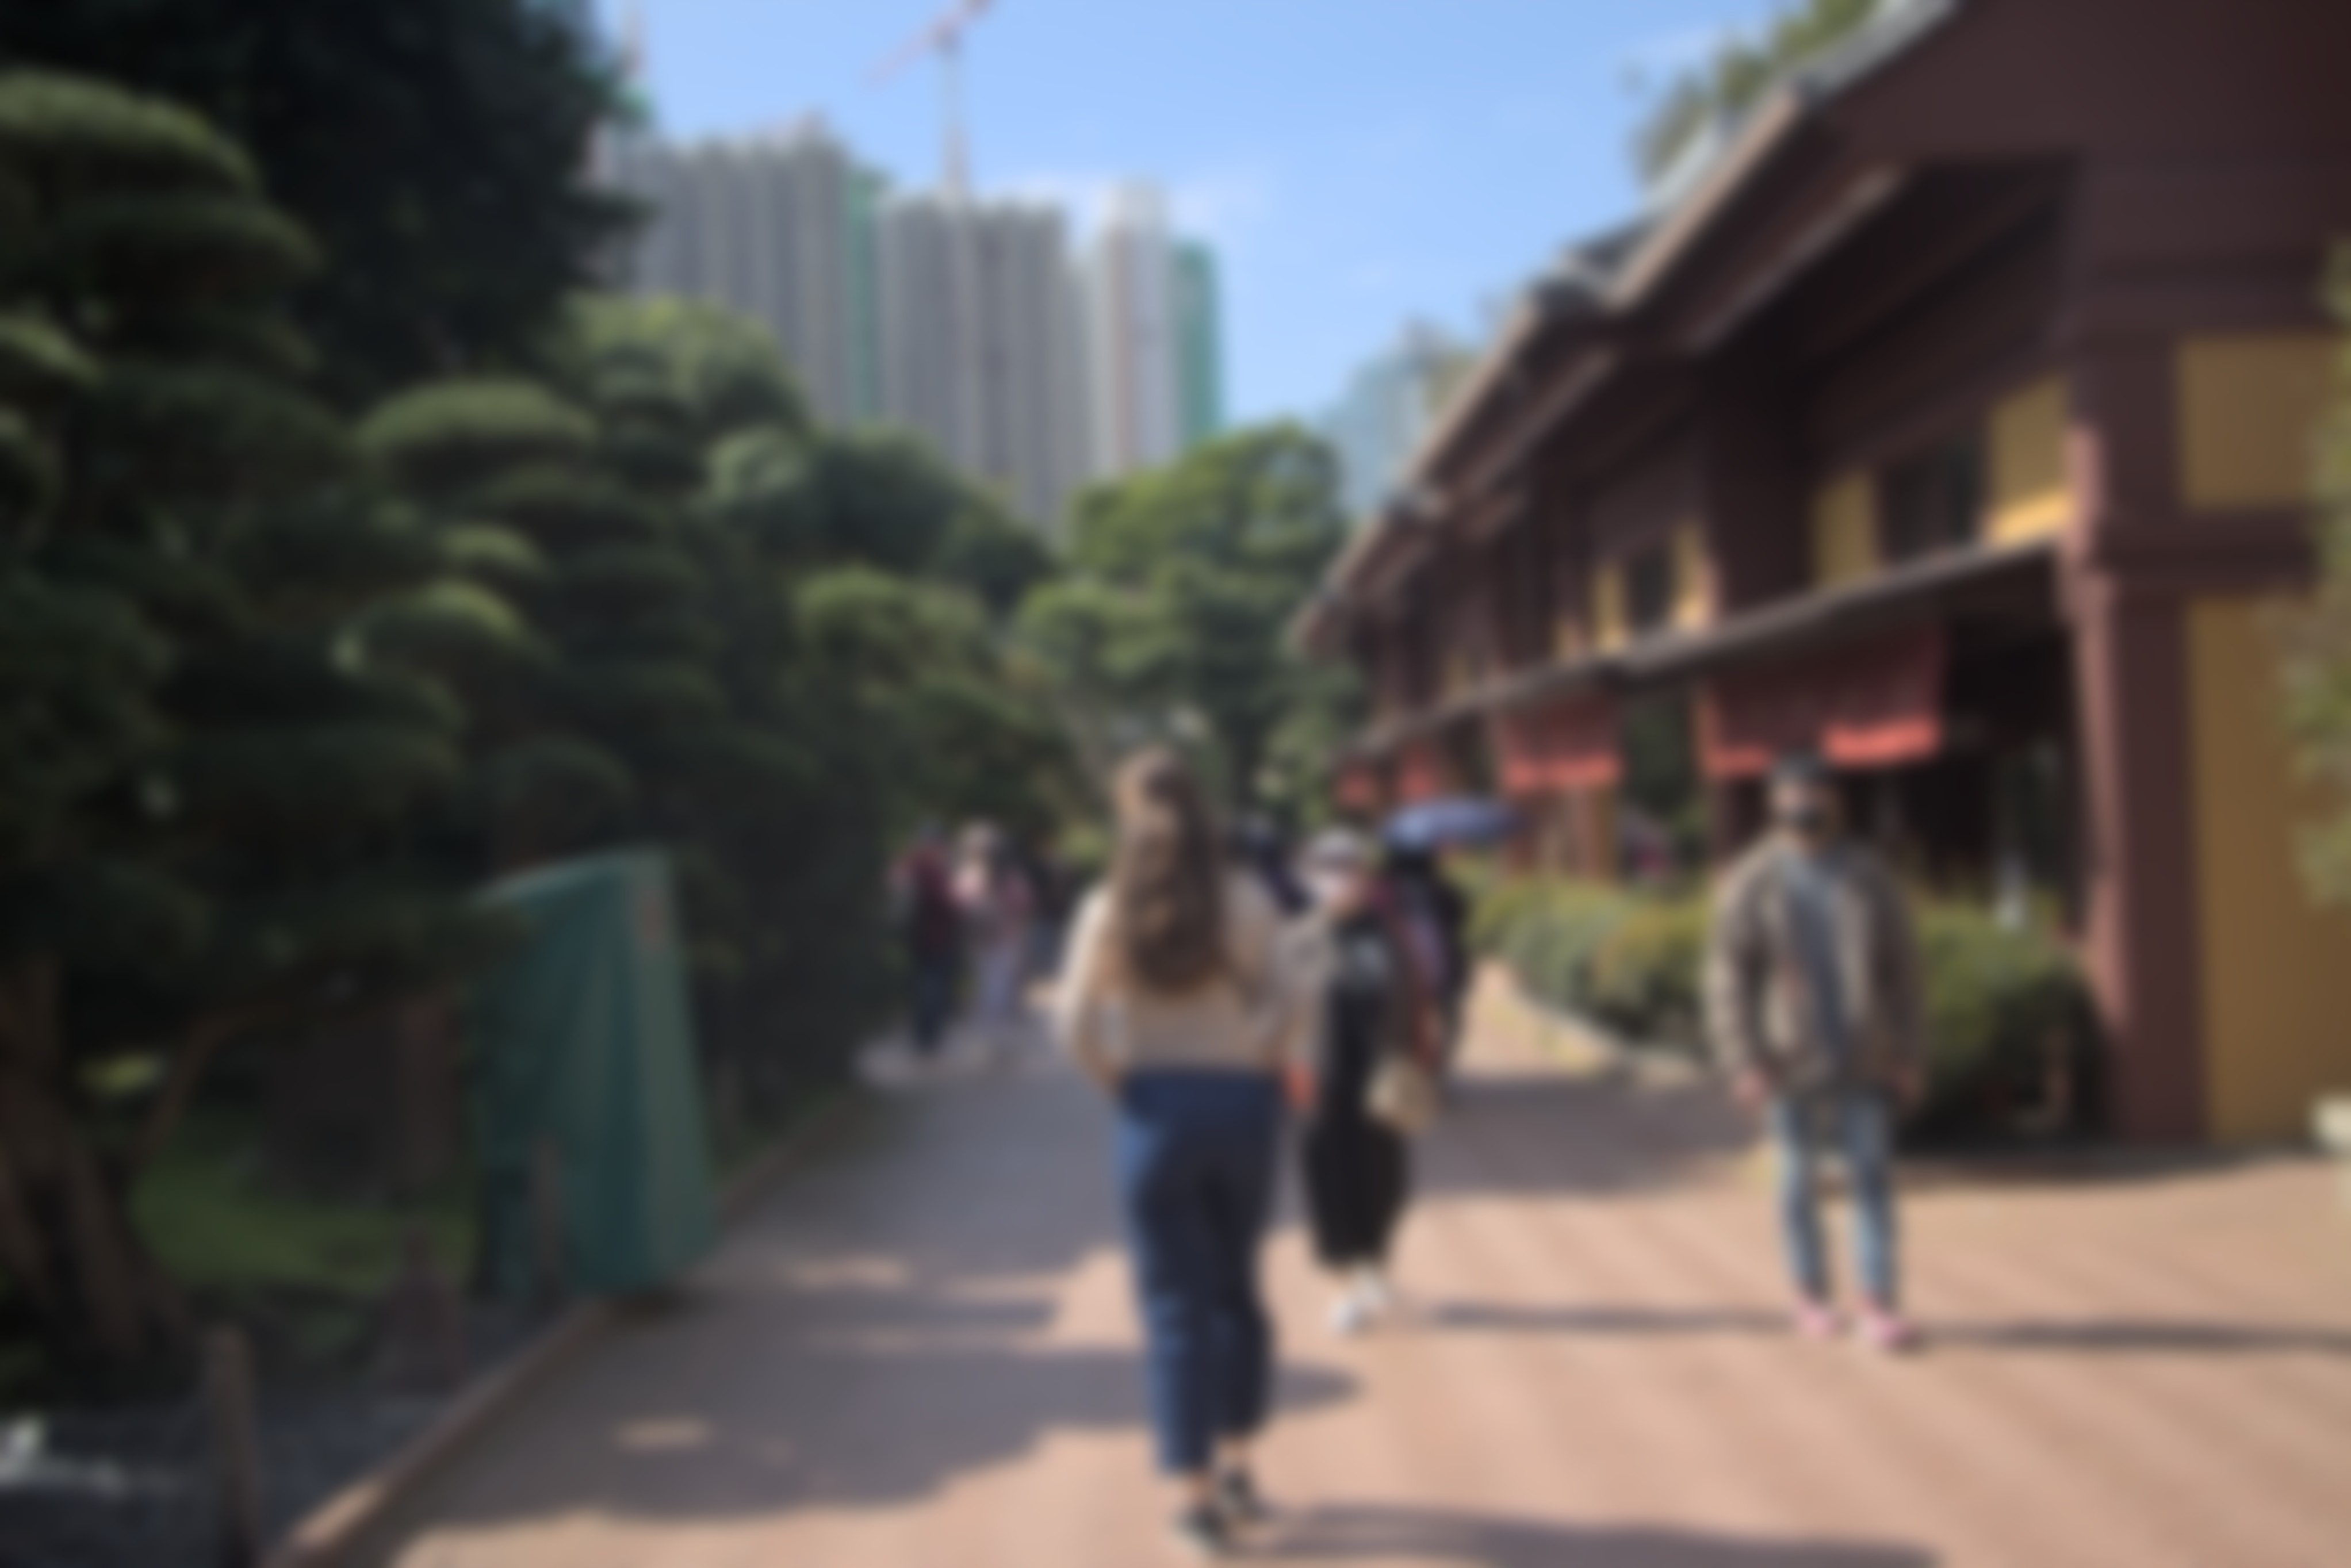
\includegraphics[width=\textwidth]{Images/Obfuscation/blurred_street.jpg}
        \caption{\centering Blurred entire image of Hong Kong street to protect privacy of citizens.}
    \end{subfigure}
    \hfill
    \begin{subfigure}{0.43\textwidth}
        \centering
        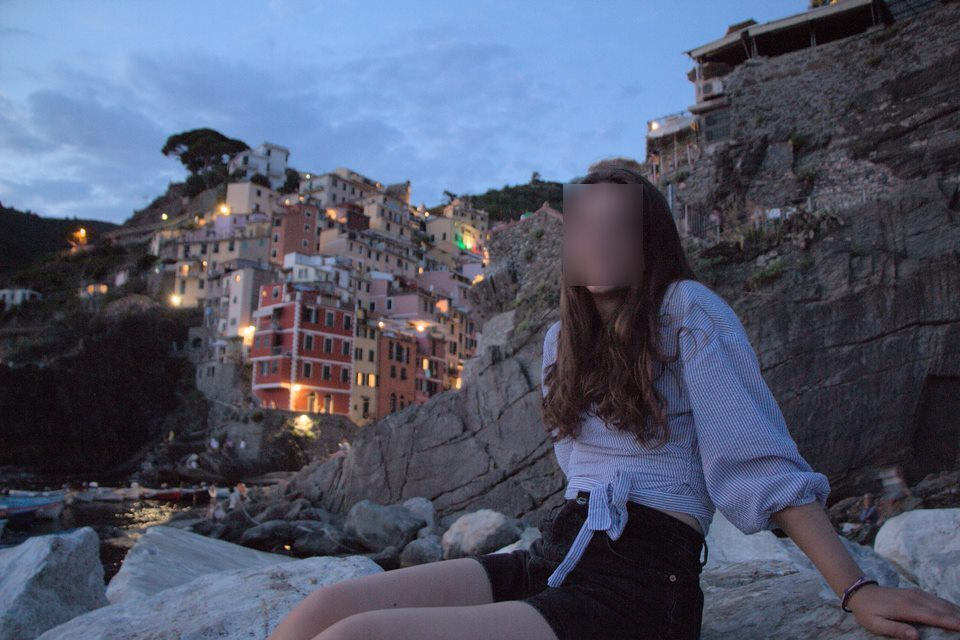
\includegraphics[width=1\textwidth]{Images/Obfuscation/face_blur.jpg}
        \caption{\centering Blurred face of individual by a sea town in Cinque Terre.}
    \end{subfigure}
    \newline

    \begin{subfigure}{0.43\textwidth}
        \centering
        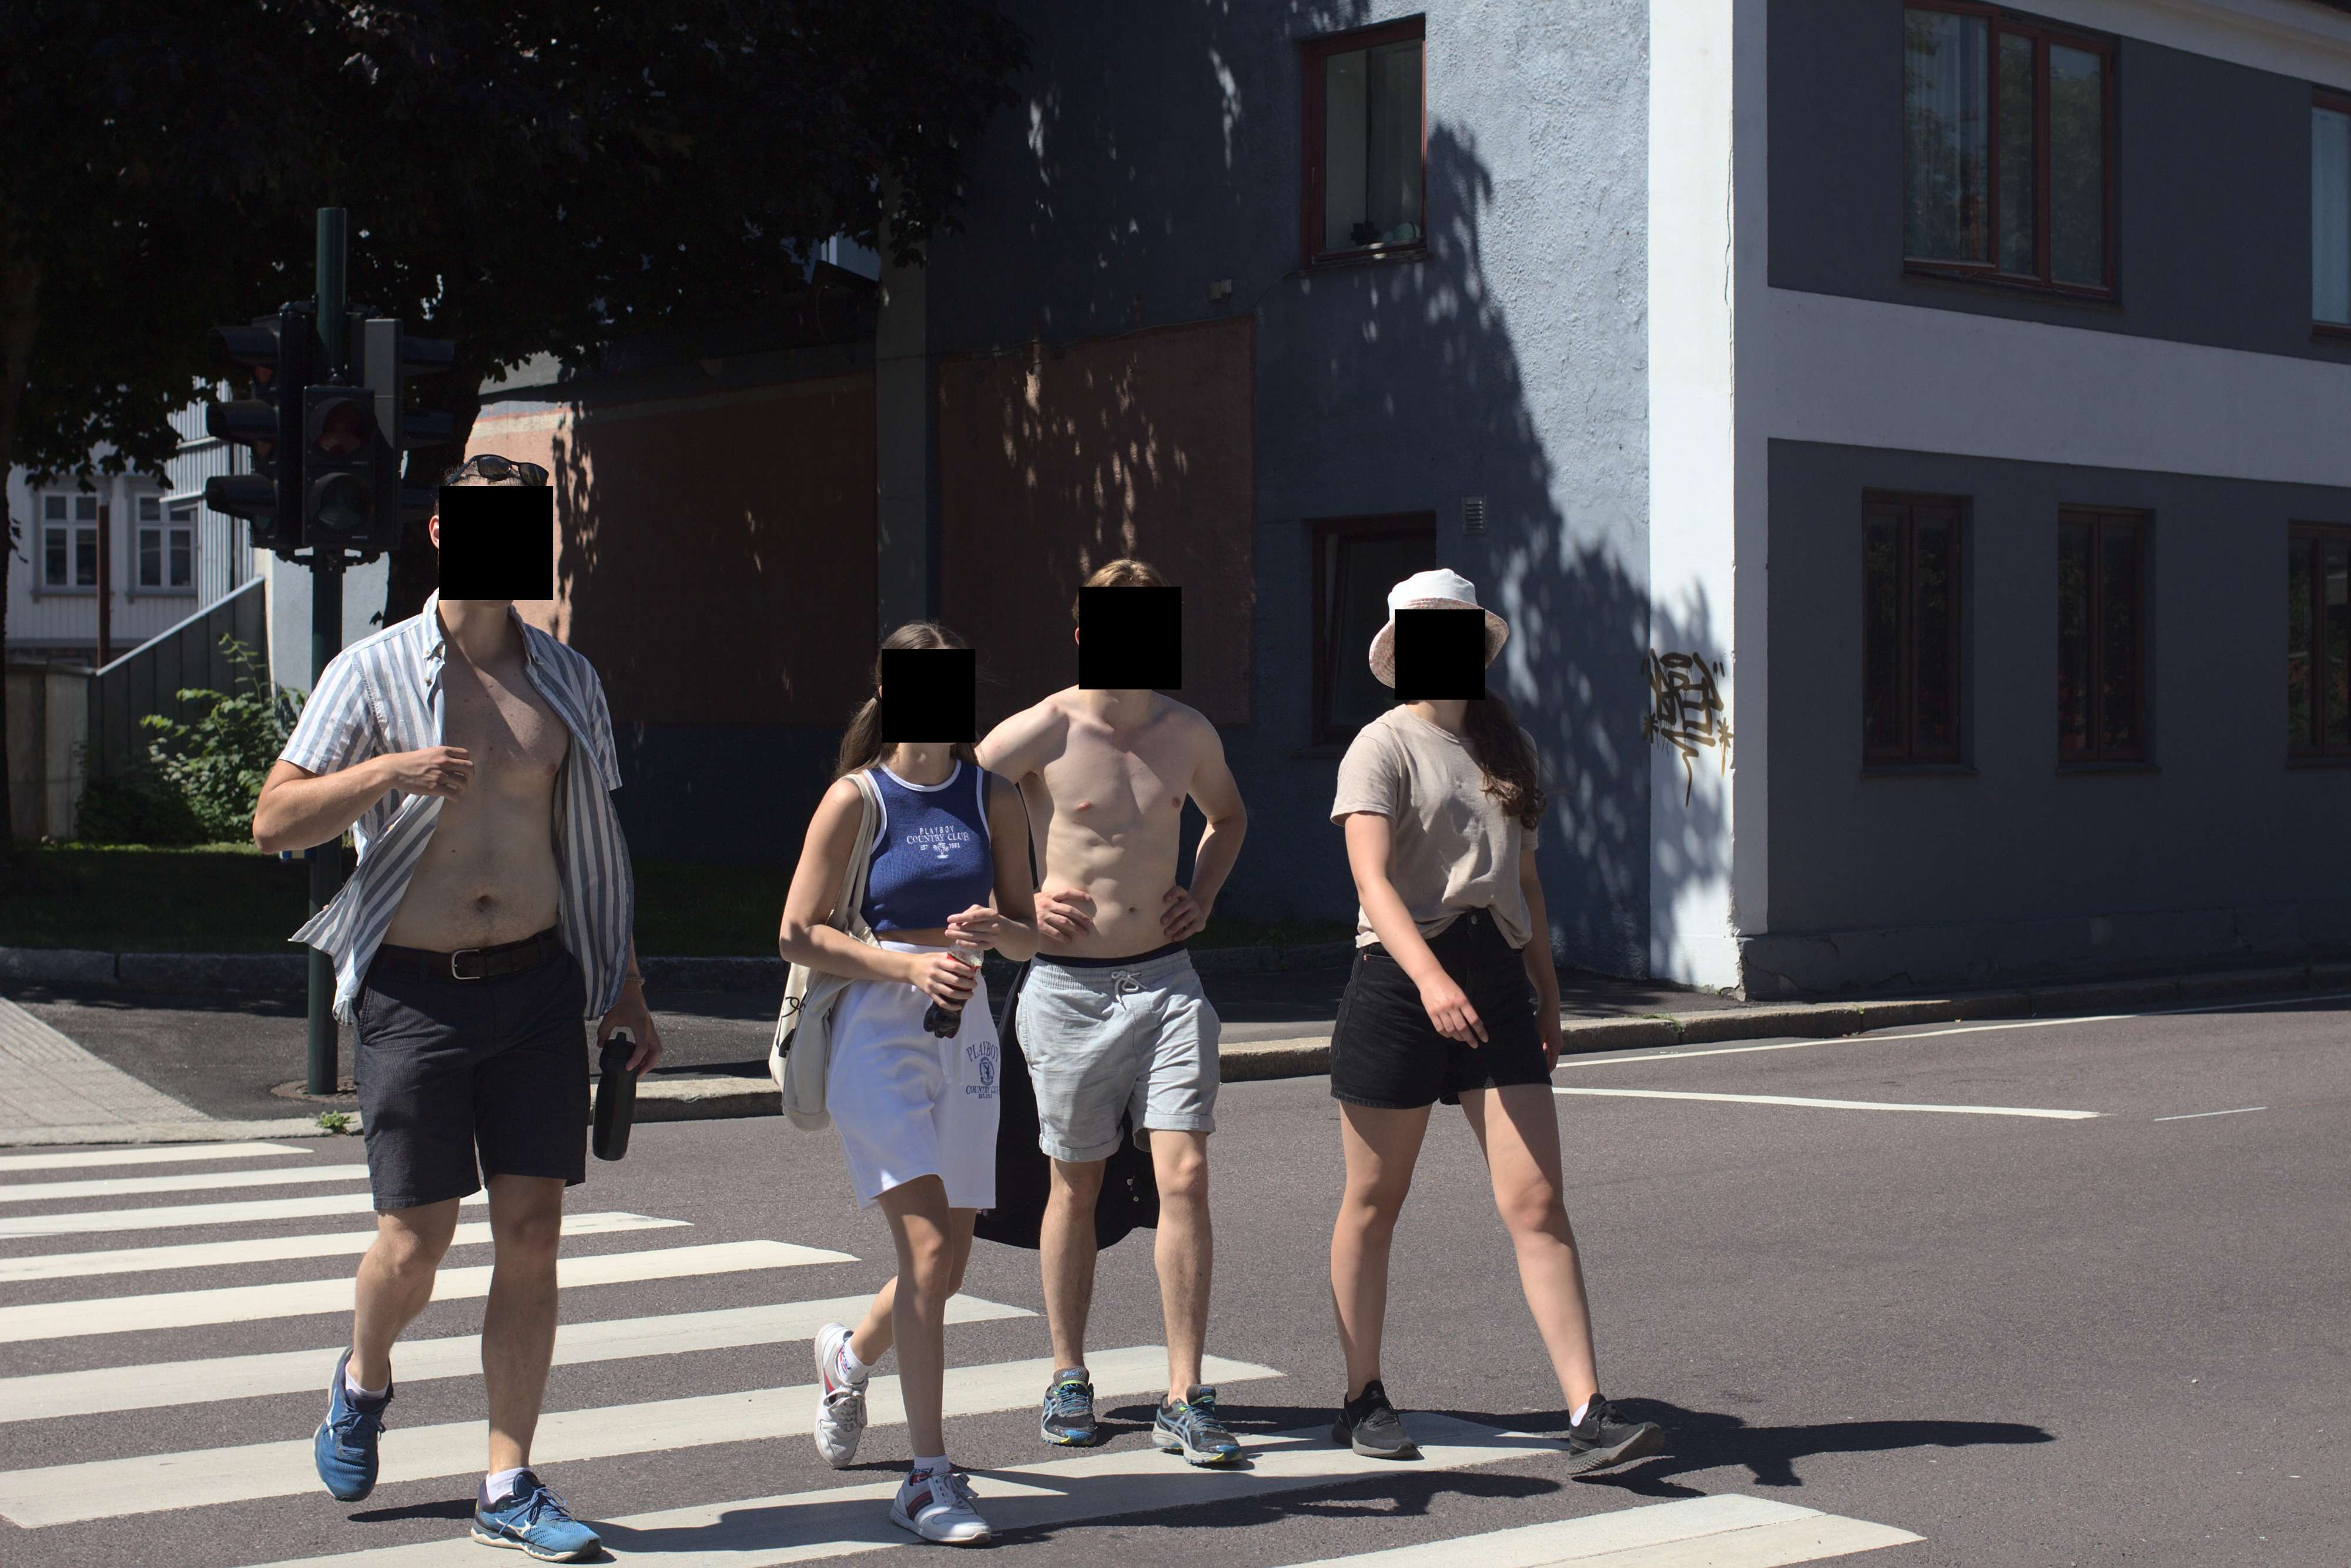
\includegraphics[width=\textwidth]{Images/Obfuscation/tonsberg_gang_masked.jpg}
        \caption{\centering Masked faces.}
    \end{subfigure}
    \hfill
    \begin{subfigure}{0.43\textwidth}
        \centering
        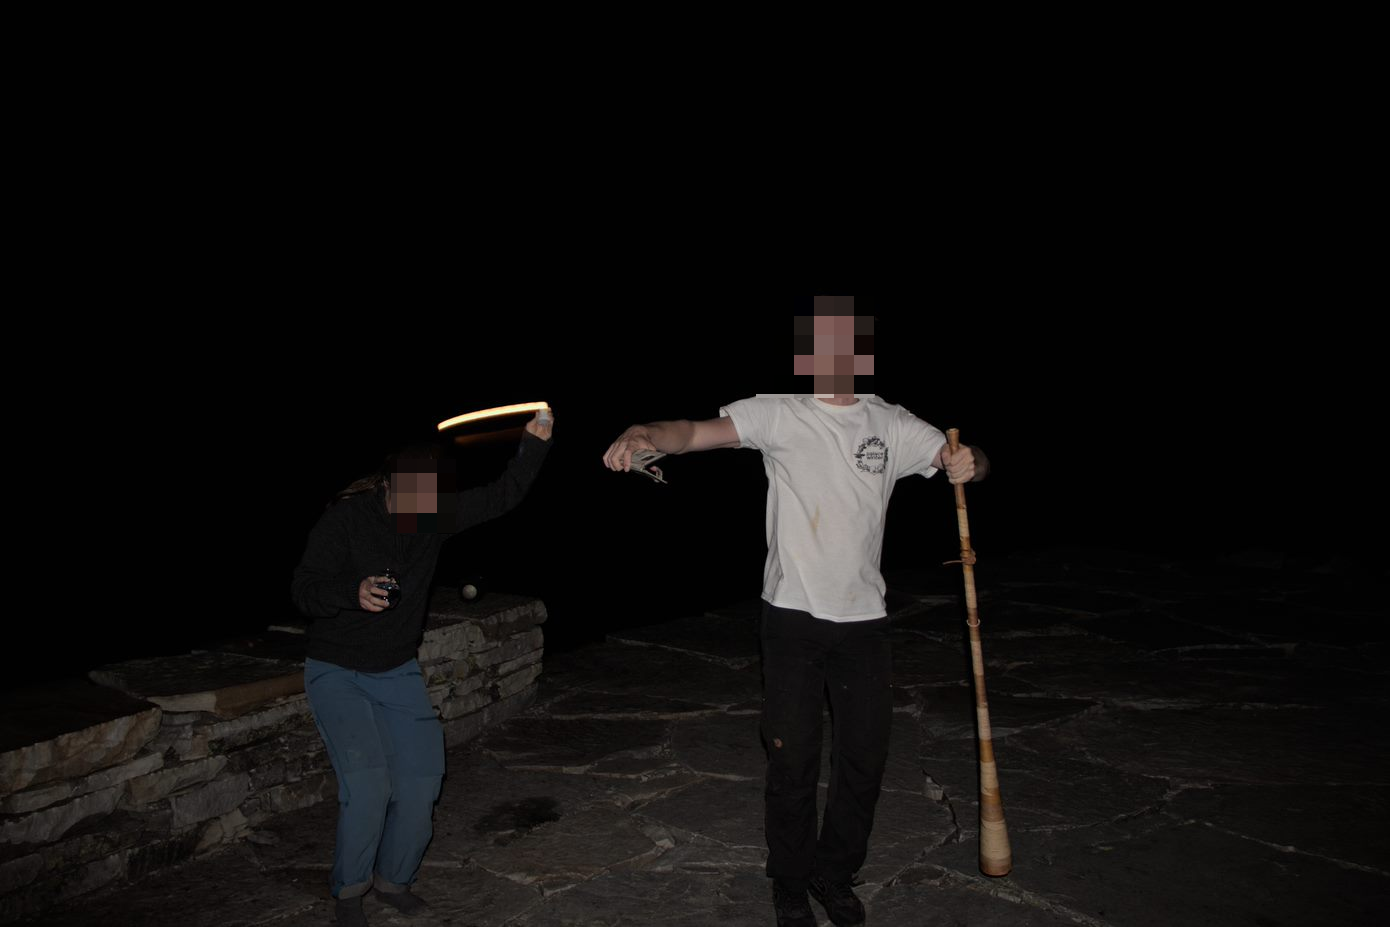
\includegraphics[width=\textwidth]{Images/Obfuscation/gausta_pixelated.png}
        \caption{\centering Pixelated faces.}
    \end{subfigure}
    \newline

    \begin{subfigure}{0.43\textwidth}
        \centering
        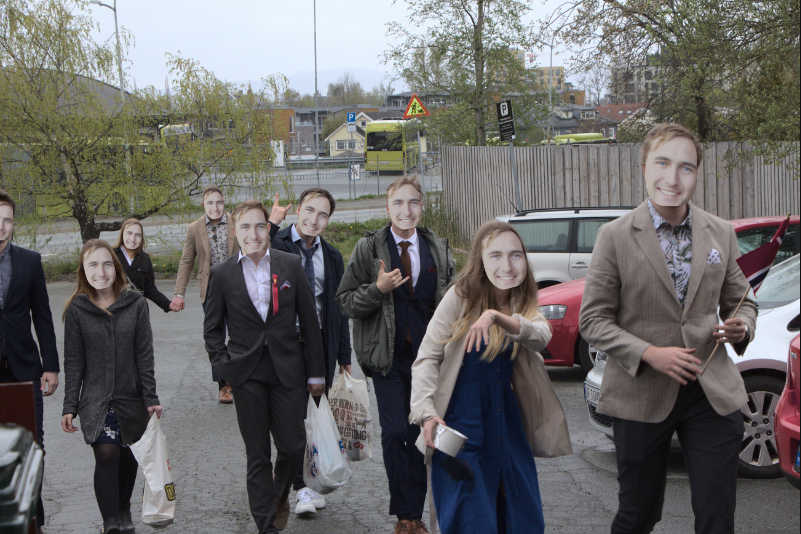
\includegraphics[width=\textwidth]{Images/Obfuscation/me_my_friends_and_I.png}
        \caption{\centering Unconventional method: replace faces. May be done as effectively as the other approaches, but is likely to be seen as an unprofesional approach.}
    \end{subfigure}
    \hfill
    \begin{subfigure}{0.43\textwidth}
        \centering
        
\includegraphics[width=\textwidth]{Images/Obfuscation/white.png}
        \caption{\centering Deleted image. This is the most effective and secure, but removes the possibility of verifying results and is unsuitable for most vision-based applications.}
    \end{subfigure}

    \caption{\centering Six Methods of Individual Privacy Preservation in Images}
    \label{fig:obfuscation_methods}
\end{figure}

K-anonymity was claimed to be a mathematically proven method for anonymyzation of personal data, but has been critizised by its successor, the l-diversity criterion, for not being robust in the events where attackers have background data (\cite{ma2007l-diversity}). Differential privacy is a statistical disclosure control algorithm to process individual data from a group to produce close-to-real outcomes without disclosing the personal data of individuals (\cite{hu2023metaverse-privacy}). Differential privacy is explained and illustrated in \ref{sec:differential-privacy}.

There has been considerable research focused on preserving privacy within the realm of machine learning (\cite{ra2023visual_privacy_techniques}). A fundamental principle shared across various use cases is that deleting data serves as the most definitive means of ensuring privacy, assuming such measures are practicable. When only non-personal data is retained, the application achieves unequivocal security concerning privacy.

\subsubsection{Federated Learning}
\label{sec:federated_learning}
In many systems relying on machine learning, being able to utilize locally stored personal data may augment the system to perform better for the situation it was created for. However, sharing this personal data with a centralized model may not be possible due to the legal bases for processing personal data (see sec:legal-bases-processing-personal-data).

Federated learning, also known as collaborative learning, is a decentralized approach to training machine learning models. It does not require exchange of data from client devices to global servers. The concept of federated learning is seen in Figure \ref{fig:federatedlearning}. 

\begin{figure}[H]
    \centering
    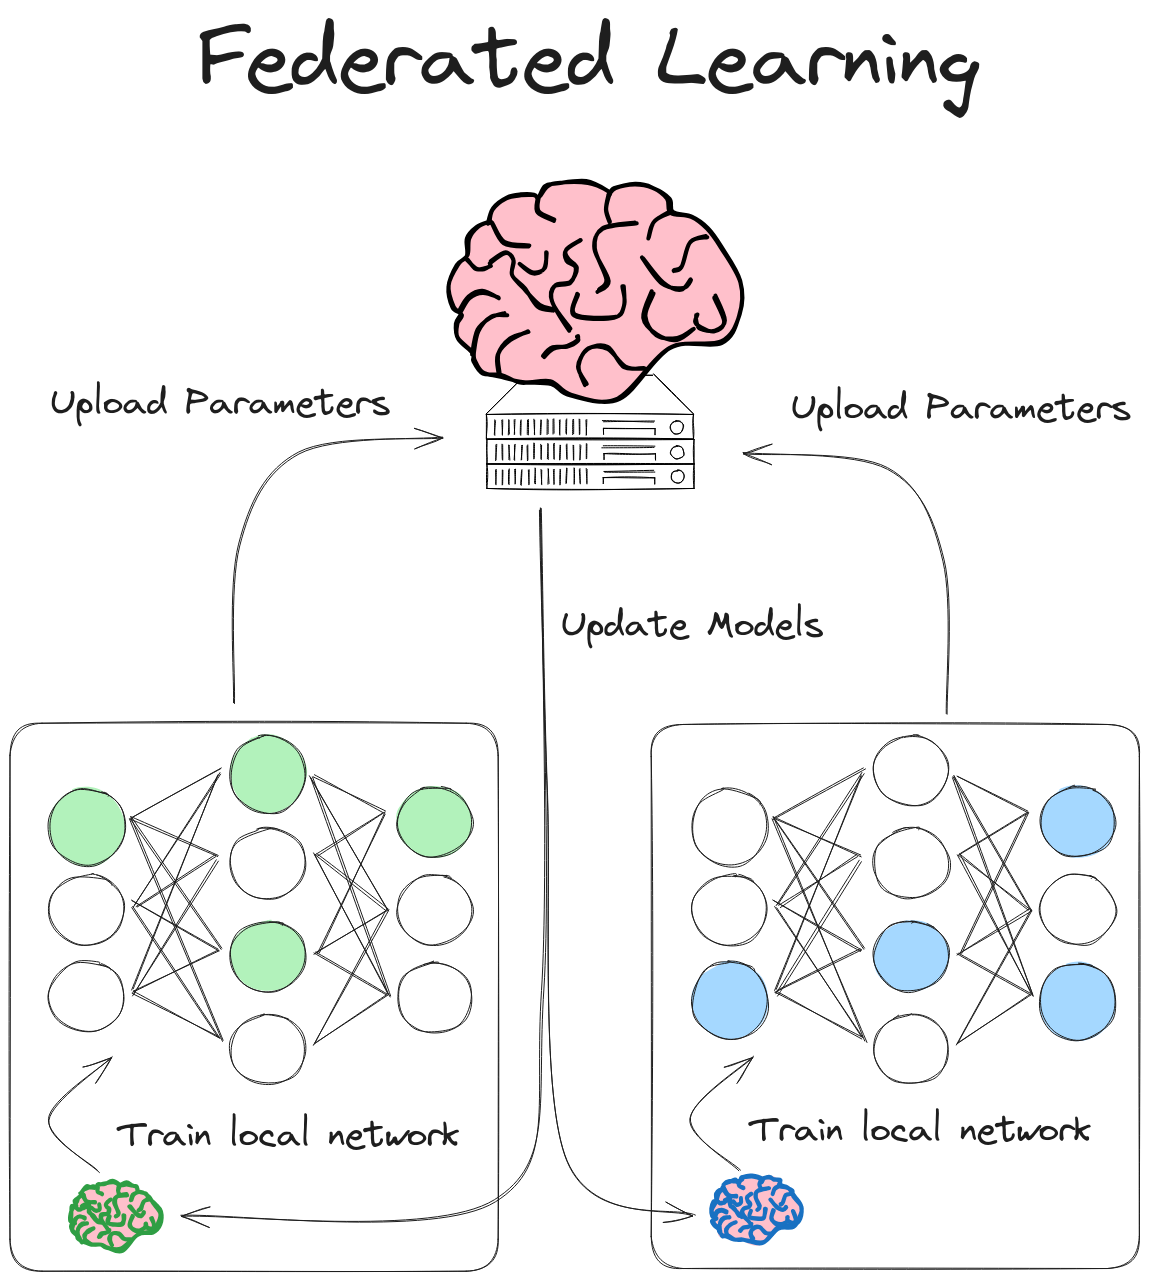
\includegraphics[width=0.75\textwidth]{Images/Diagrams/FL_updated.png}
    \caption{\centering The Federated Learning Concept}
    \label{fig:federatedlearning}
\end{figure}

\newpage Federated learning is described in the article of \citeauthor{an2022federatedlearninghealthcare} (\citeyear{an2022federatedlearninghealthcare}): 

\begin{myquote}
    A central entity manages the learning process and distributes the training algorithm to each participating data holder. Each participant generates a local model trained with their private data and shares the resulting parameters with the central entity. Finally, the central entity employs an aggregation algorithm to combine the parameters of all local models into a single global model.
\end{myquote}

In summary, FL enables the training of ML models locally (at the location of the data) and only shares the resulting model, which is not reverse-engineerable, with the requesting party. Therefore, FL avoids the need to share the private datasets and sensitive data to others, preventing exposition to entities conducting studies and enabling data usage for broader purposes (\cite{re2021servertoclientml}). 

The FL process is reliant on having ground truth data on the edge for training the models correctly, but obtaining the ground truth for edge device models operating on \textit{visual data} is difficult. The way this may be achieved, is by having a powerful edge device perform the inferences with a computationally expensive but accurate model, and using the inference results of this model as the ground truth for training a separate, possibly faster and less computationally expensive model to replace the other at a later stage. Otherwise, one could also perform the training under conditions where the ground truth is known, for example by manually inputting the number of people in an area, then having the model learn to arrive at the same count based on the camera input.

Improvement of machine learning models devices in the healthcare industry present challenges due to the sensitive nature of medical data from patients. Centralized training of machine learning models may violate laws such as the GDPR, because of the way data is being collected and used unbeknownst to the data subject (\cite{an2022federatedlearninghealthcare}). To tackle these issues, \citeauthor{an2022federatedlearninghealthcare} (\citeyear{an2022federatedlearninghealthcare}) proposes the usage of FL\footnote{Specifically, the FL method described in the works of \citeauthor{ya2019federatedMLconcepts}(\citeyear{ya2019federatedMLconcepts})} to tackle these issues.

Furthermore it should be noted that FL is a method to deal with the existential nature of data in edge computing devices, best described as \textit{isolated islands}, and to use the data on edge devices before it is deleted or obscured, to improve the intelligence of the devices in privacy preservant and protective way. An important measure to take in the development of FL models is to ensure that the models are not reverse-engineerable, as the models may contain personal data. This is done by adding noise to the data, which makes it impossible to backtrack the data to the individuals. This may be done by a method such as differential privacy, which is discussed in Section \ref{sec:differential-privacy}.

\subsubsection{Differential Privacy}
\label{sec:differential-privacy}
Regulations regarding personal data also applies to the events where pieces of information are aggregated to identify a person. The concept of differential privacy is to make data of individuals privacy-preservant through describing them as a group. Data from the group of people may be used, but without the possibility of backtracking the information to certain individuals. See Figure \ref{fig:differential-privacy}.

In more technical terms: Differential privacy is a statistical disclosure control algorithm to process individual data from a group to produce close-to-real outcomes without disclosing the personal data of individuals (\cite{hu2023metaverse-privacy}). This means that the data is processed in a way that the results are close to the real results, but the data is not disclosed. This is done by adding noise to the data, which makes it impossible to backtrack the data to the individuals.

Differential privacy is particularly pertinent in the context of federated learning. In this approach, client devices add controlled noise to their model updates—or weights—before sending them to a centralized server. This noise addition prevents the server from being able to infer individual-specific information from the model updates. The degree of noise is regulated by a privacy parameter, often referred to as a privacy budget. This strategy allows the central server to aggregate these noisy updates from all participating nodes to update the global model. Contrary to the original statement, the noise is not removed but rather managed in such a way that the aggregated model maintains utility while protecting individual privacy (\cite{sh2023RolwOfWeightTransmissionProtocolinML}).

Note that differential privacy is a definition, not an algorithm (\cite{dw2011DifferentialP}). In other words, we can have many different algorithms that satisfy the privacy demands for a given use case. For example, \citeauthor{dw2011DifferentialP} mentions the Laplace mechanism (outlined in the same authors works from \citeyear{dw2006noise2sensitivity-laplace}) as an optimal mechanism for answering “tally” type questions differentially privately (\citeyear{dw2011DifferentialP}). For more advanced situations, other algorithms, such as the method outlined by \citeauthor{bl2011learning-privacy} (\citeyear{bl2011learning-privacy}), are more suitable (\cite{dw2011DifferentialP}).

The big tech giants like Apple, Google and Microsoft employ differential privacy in their data collection and analysis to ensure the privacy of their users. Differential privacy is a method to ensure that the data is not personal, and thus not subject to the GDPR.

\begin{figure}[H]
    \centering
    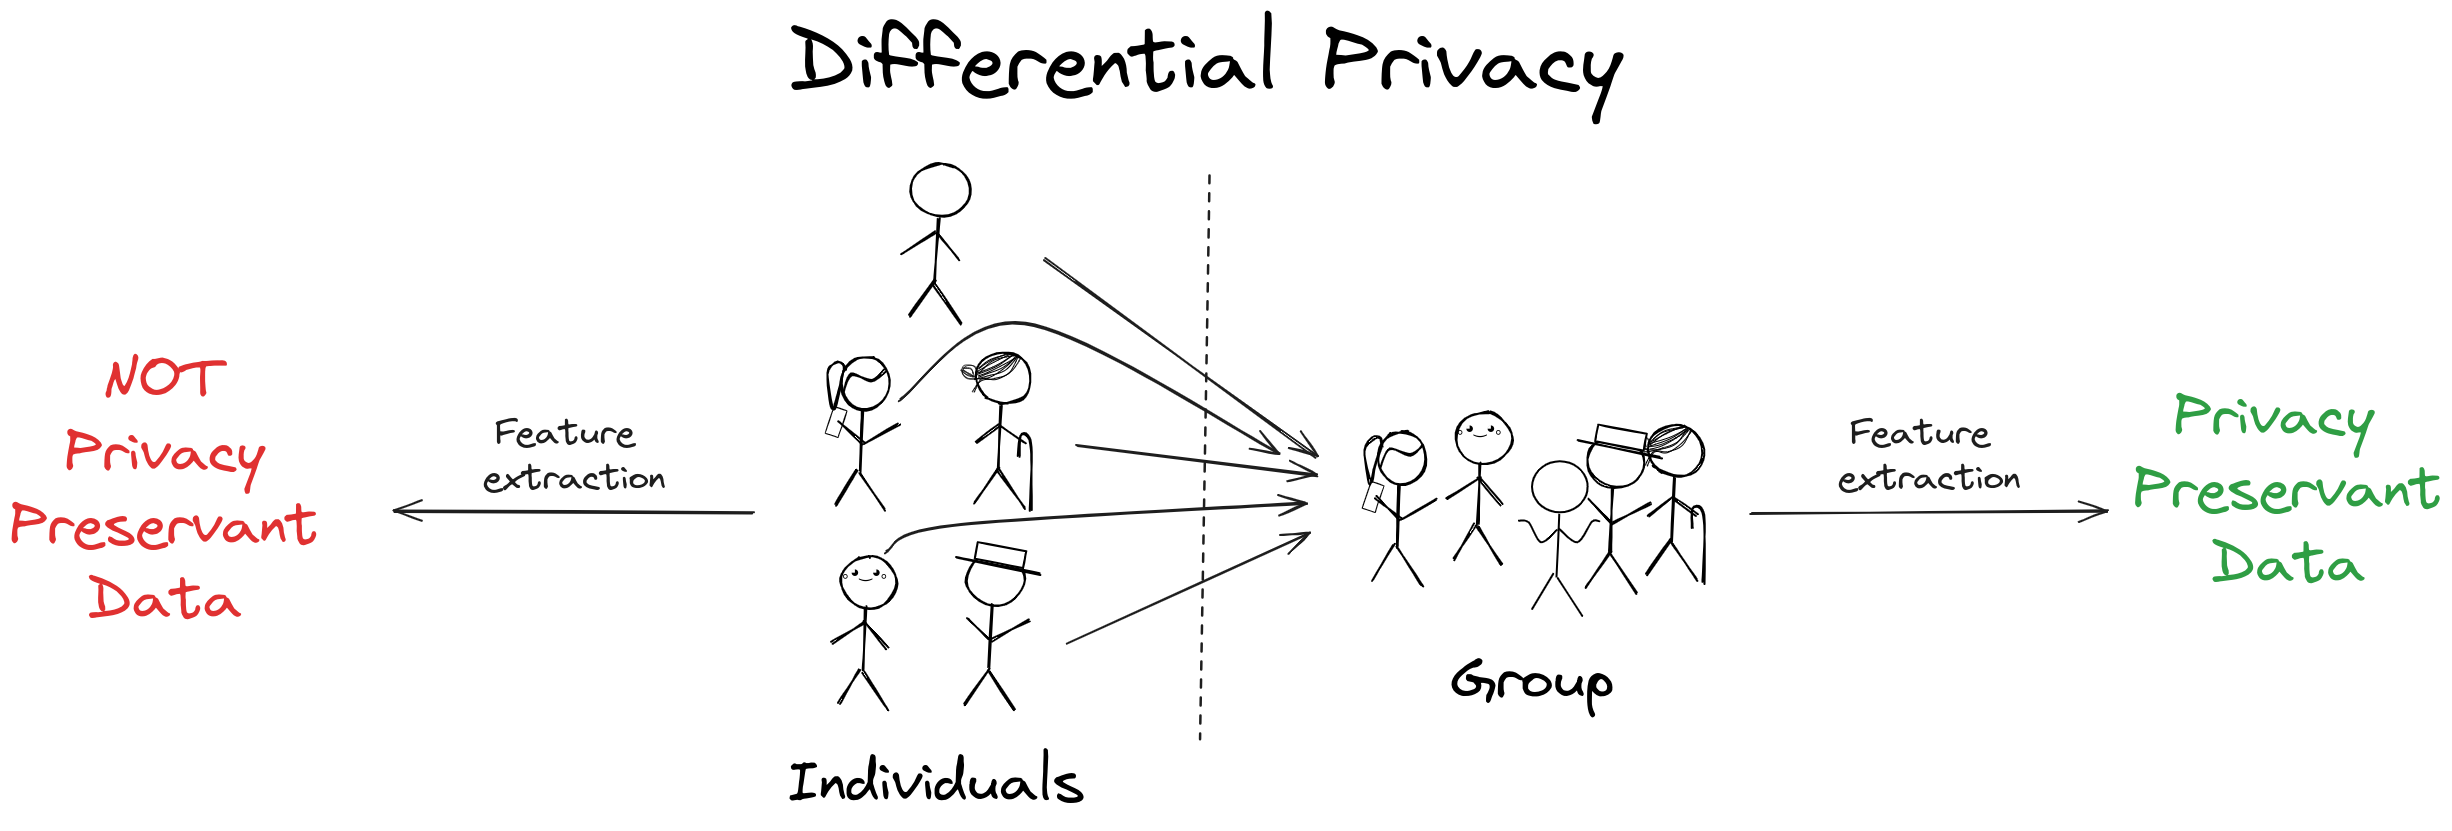
\includegraphics[width=\linewidth]{Images/Diagrams/differential-privacy.png}
    \caption{\centering The Differential Privacy Concept}
    \label{fig:differential-privacy}
\end{figure}

\subsubsection{On-Device Processing}
According to \citeauthor{hu2022accurateobjectdetectionatedge} (\citeyear{hu2022accurateobjectdetectionatedge}), there are four methods for running tasks on resource-constrained edge computing devices. This is relevant in applications where user's concerns for privacy increases if data is directly transmitted to a server. These methods are seen in Table \ref{tab:methods_to_run_tasks}, and explained discussed in the following paragraphs.

\begin{table}[H]
    \centering
    \renewcommand{\arraystretch}{1.5} % Increase vertical padding
    \setlength{\tabcolsep}{1em}
    \begin{tabular}{|l|l|l|}
        \hline
        \rowcolor{gray!25}
        \textbf{Method} & \textbf{Advantages}                & \textbf{Disadvantages}  \\ \hline
        Data encryption & Privacy protection                 & Much bandwidth          \\
                        & Fast calculation                   &                         \\ \hline
        Traditional ML  & Little resource consumption        & Relying on the Internet \\
                        &                                    & Poor robustness         \\ \hline
        Task sharing    & Reducing stress on a single device & Much bandwidth          \\
                        &                                    & Large latency           \\ \hline
        Deep learning   & Privacy protection                 & High resource           \\
                        & High robustness                    & consumption             \\ \hline
    \end{tabular}
    \caption{\centering Comparison of Methods for Running Tasks on Resource-Constrained
        Edge Computing Devices (\cite{hu2022accurateobjectdetectionatedge})}
    \label{tab:methods_to_run_tasks}
\end{table}

\paragraph{Data Encryption}
The first method, data encryption, would be one way of transmitting images in a more secure way. This should be done in a lossless way to maintain the image quality to preserve the accuracy of the detectors. Doing so is not trivial, and is a research field on its own. A few methods that may function well, e.g. blurring only the faces, are discussed in Section \ref{sec:obfuscation}.

\paragraph{Traditional Machine Learning}
The second method for running tasks on resource-constrained devices is to implement the less computationally expensive traditional machine learning methods. Unfortuneately, this is a unprefferable solution in many situations due to their lack of accuracy compared to the deep learning models. This is displayed in Figure \ref{fig:object_detect_20_years_improvement}). Here, we see the mean average precisions (mAPs) have skyrocketed since the introduction of neural networks as backbones for object detection algorithms. Note that the best performing algorithm in 2015, the year after COCO was introduced, scored a mAP50-95 of 35.9. This value has nearly doubled with the development of YOLOv4, and has been further improved with the more advanced transformer technologies thereafter. 

Traditional machine learning algorithms may, however, be a good option for devices with low computing power and memory resources as they are generally low-demanding and may be easier to understand\footnote{Neural networks struggle with explainability and are often referred to as black boxes}. The traditional methods are most applicable to use cases with clear, deterministic logic. Traditional machine learning methods were the most prominent prior to 2014, while deep learning based detection models have been the completely dominant approach to image recognition tasks. To achieve similar accuracies to those of the deep learning models but with the low computational demands of traditional machine learning, one might consider to investigate the field of tinyML, which was scoped out of this thesis \ref{sec:scope_tinyML}. Some considerations are, however, added in appendix \ref{app:tinyML} due to their relevancy to resource-constrained edge computing devices, a topic considered bordering to the thesis.

\begin{figure}[H]
    \centering
    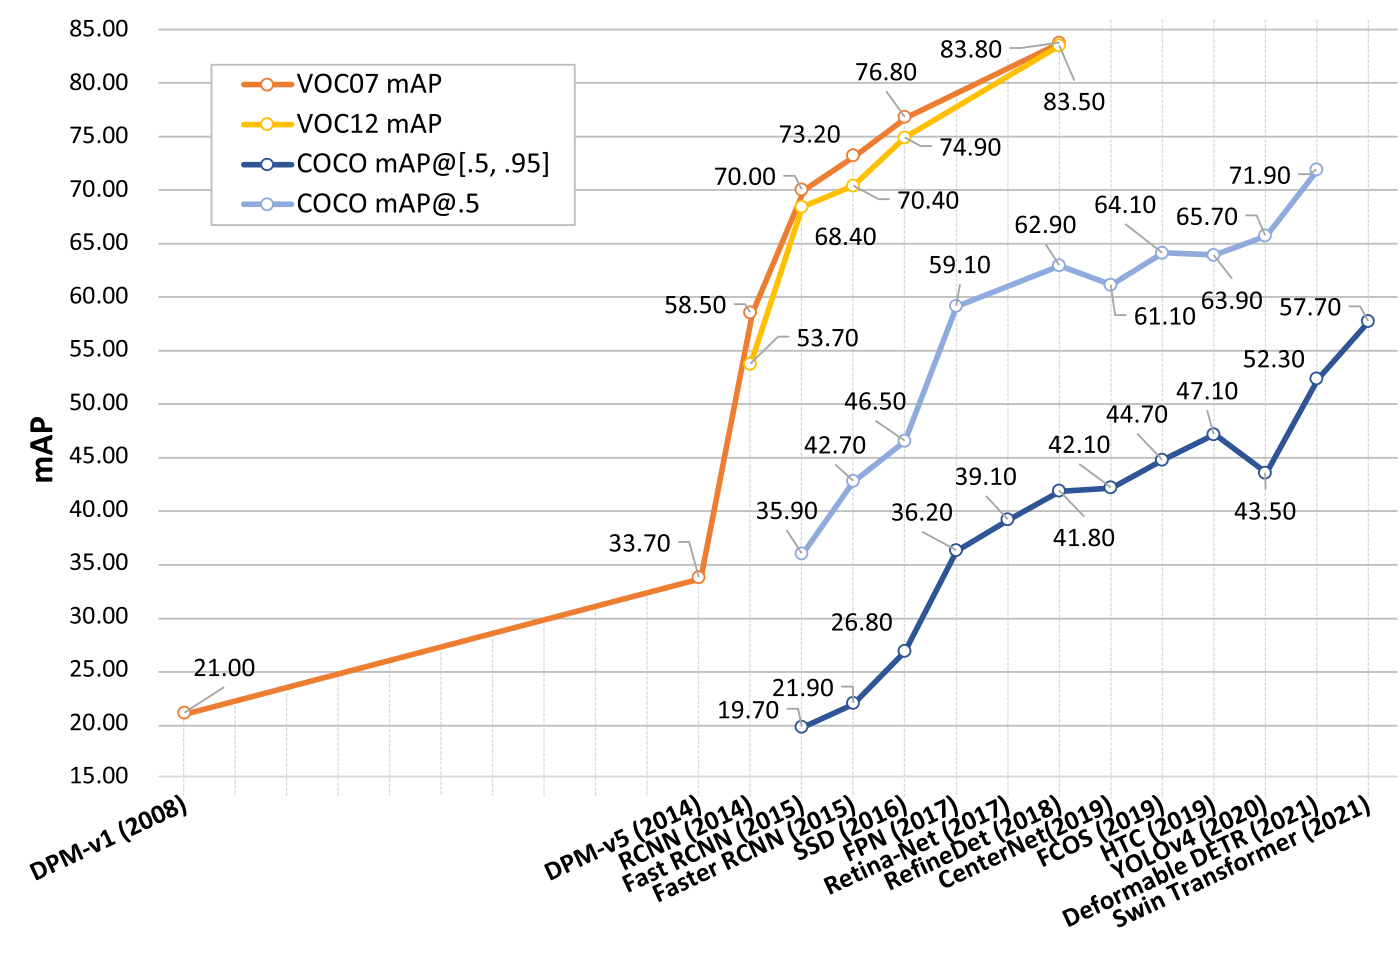
\includegraphics[width=1\linewidth]{Images/Diagrams/object-detection-improvements.png}
    \caption{Accuracy Improvement of Object Detection on VOC07, VOC12, and MS-COCO datasets (\cite{zou2023object_detection_in_20_years})}
    \label{fig:object_detect_20_years_improvement}
\end{figure}

\paragraph{Task Sharing}
The third method, sharing the workload over multiple devices, is not an uncommon practice in technology. See for example Eufy's solution with a home-base device in Section \ref{sec:eufycam}), where the camera devices take images and send them to a more powerful computer for processing. This approach reserves privacy, because the images are never sent outside of the local network, and it can be implemented with simple TCP/IP\footnote{Transmission Control Protocol/Internet Protocol is a set of standardized rules that allow devices to communicate with each other on a network.} communication. 

Task sharing results in low latency, fast networks, but introduces (1) the need of having a central hub, (2) extra work of setting up the transmission protocols, (3) another source of error and (4) the need to encrypt/decrypt images prior/post transmission to ensure security. However, due to periodically scarcity in the availaility of specialized hardware such as GPUs, this approach could be useful since a single GPU per facility may achieve a higher throughput than processing large data on the CPUs of multiple edge devices.

\paragraph{Deep Learning}
As opposed to traditional machine learning,
This section outlines some methods to retain the privacy of individuals by using different sensors or implementing neural network on the edge devices, often referred to as on-device processing or edge computation. Which term of on-device processing and edge computation is used may be dependent on which aspect of the concept the author chooses to emphasize; the actual process that is happening on a device, or the architectural decision of making the computation on the edge.

\subsubsection{Depth Cameras}
A widely used approach within the domain of anonymous fall detection, is to use of RGB depth cameras to capture depth information (\cite{wa2020elderly_fall_detection_meta}). As only depth information is captured, the data remains completely anonymous from the start.

\subsubsection{Deletion of Images}
\label{sec:deletion_of_images}
In an investigation of an already existing internet of things (IoT) system for wildlife monitoring: 'Where's The Bear', relying on motion-triggered cameras, three challenges of visual systems in such applications were discussed \cite{el2017WTB}. The drawbacks were (1) the transmission of enormous numbers (sometimes millions) of images over low-bandwidth networks, which tend to happen in automatically (motion-) triggered applications, (2) motion sensors triggered by weather conditions or by animals that were not of interest, and (3) redundancy of images taken of the same individual animal. While the 2nd and 3rd drawbacks are not applicable to this project, the 1st is.

\citeauthor{el2017WTB} proposed a solution to this challenge: edge computing. Edge computing, also referred to as on-device processing, encapsulates similar concepts but emphasizes slightly different aspects of the computing approach. While \textit{on-device processing} specifically indicates that the computational tasks are carried out directly on the device itself, \textit{edge computing} underscores that these tasks are performed close to the data sources, i.e., at the \textit{edge} of the network.

The deployment of visual systems in public spaces presents challenges related to privacy, not only because of the immediate access to private data, but also due to the recent breakthroughs in object detection allowing the extraction of sensitive information from visual data. The altogether only completely safe way to ensure complete and total privacy of data, is to not have the data at all.

Edge computing and on-device processing allows for the image is obscured or deleted right after analysis without ever leaving the edge device. In this way, only the anonymous analysis results are communicated online. This would mean that the personal data (1) exists \textit{just} while the analysis is running, (2) is never sent online, and (3) is thus a lot less vulnerable to attacks. The perpetrator's device would need to be physically connected to the device and the attack would need to happen in real time. In those cases, the perpetrator could quite likely just as well take the photo himself. This is an approach to achieve low-latency, high bandwidth, high availability, low cost communications and fast response to/from the sensors.

The images would in some cases benefit in multiple ways from being obscured instead of deleted. This approach is discussed in the following paragraph.

\subsubsection{Obfuscation}
\label{sec:obfuscation}
Another way to remove the privacy concern is by obscuring the images after analysis in such a way that individuals may never be identified.

Obfuscation is the action of making something obscure, which means to conceal or make unclear. To obscure an image is often used interchangeably with “to blur”, but they are not the same. To blur means to make something indistinct or hazy, and is a specific method of obscuring an image. Other methods for obscuring an image is masking or pixelate the faces of individuals. These methods are illustrated in Figure \ref{fig:obfuscation_methods}.

\paragraph{Blurring the Faces}
In a \citeyear{ma2019fall_anonymous} study, faces were detected with a thermal-detecting camera and then photos were captured with an RGB camera, blurring the area the face was detected by the thermal camera (\citeauthor{ma2019fall_anonymous}). This approach is privacy preservant as long as all faces are blurred, but may fail if the algorithm does not detect all faces. In those cases, however, most humans would likely also struggle to identify a person based on the face. On the contrary, in many cases, blurring the entire image would compress the image, making it faster and easier to transfer, and be the faster option than having to detect all faces in an image.

\paragraph{Perceptions of Privacy Enhancement Methods}
A questionnaire study of 328 students indicated that blurred images were not considered by the students to provide satisfactory privacy protection (\cite{ed2012privacy_review}). Participants were given 18 randomly ordered videos, and were asked to rate the privacy on a Likert\footnote{Likert scale: A scale of odd options, where the participant may answer a neutral middle-option and distribution should be equally distributed in both directions thereafter. An often used questionnaire scale in psychology research.} scale from 1-5. The obfuscation methods, or privacy enhancements as they called them, and the results are displayed in Figure \ref{fig:ed_results}. The results show that blurred images were only considered privacy preservant for 23 percent of participants. Regardless, an important notion is that the images of this survey are from within a private home, posing higher demands and expectations with regards to privacy than what is typically done in a more public space.

\begin{figure}[H]
    \centering
    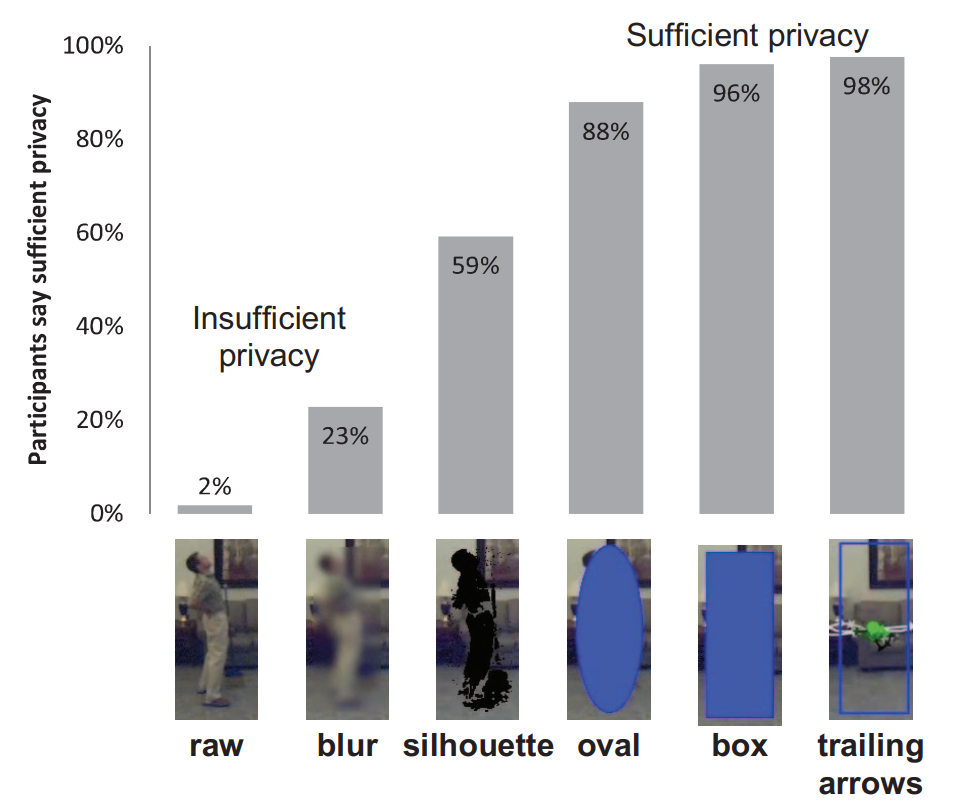
\includegraphics[width=0.6\textwidth]{Images/ed2012results.png}
    \caption{\centering Privacy Enhancements Methods in the Study of \citeauthor{ed2012privacy_review} (\citeyear{ed2012privacy_review})}
    \label{fig:ed_results}
\end{figure}

\subsection{Ethical Considerations in the Development of Person Positioning Technologies}
\label{sec:ethics_localization_tech}

As we advance the capabilities of technologies such as YOLOv9 for person localization, it becomes imperative to consider the ethical implications of our developments. The narrative of George Orwell's dystopian novel \textit{1984} serves as a reminder of the potential societal consequences of intelligent, extensive and automated surveillance. Orwell's portrayal of a society where history is constantly rewritten and individual privacy is obliterated highlights the dangerous path we might tread if these technologies are misused by those in control of political power.

"The Party seeks power entirely for its own sake. We are not interested in the good of others; we are interested solely in power, pure power." (\cite{orwell1984}). This may remind of some politicians, i.e. american presidents, who may decide to deploy person localization devices to keep population under control while tightening the grip on the population...

\subsubsection{Joseph Redmon Quit Computer Vision Development}
Joseph Redmon, the creator of the initial versions of YOLO, decided to cease his work on the project due to its military applications. This illustrates a profound ethical stance. Redmon's choice underscores the responsibility of developers in considering the broader impacts of their work. The resignation marks a critical point in the discourse on the moral responsibilities of researchers and developers in the field of artificial intelligence and machine learning. The discussion of how to responsibly regulate and develop AI applications is still ongoing, and the decisions made by individuals like Redmon are crucial in shaping the future of the field. 

Joseph Redmon's Twitter Posts:

\begin{myquote}
    I stopped doing CV research because I saw the impact my work was having. I loved the work but the military applications and privacy concerns eventually became impossible to ignore. (\cite{re2020twitter_feb}).

    But basically all facial recognition work would not get published if we took Broader Impacts sections seriously. There is almost no upside and enormous downside risk. (\cite{re2020twitter_feb}).

    [...] I bought in to the myth that science is apolitical and research is objectively moral and good no matter what the subject is. (\cite{re2020twitter_feb}).

    If you worked in a knife factory and a guy came in and thanked you for making knives because he killed many people with those knives and then he showed you a video of himself killing people with a knife you made how would you feel then about working in your knife factory?  (\cite{re2020twitter_june}).
\end{myquote}

\subsubsection{Philosophical Perspectives}
Immanuel Kant's deontological ethics emphasizes the importance of adhering to moral rules or duties. According to Kantian philosophy, actions are morally right if they are in accordance with a moral rule or principle, regardless of the consequences. A Kantian ethics viewpoint slightly adjusted to the development of localization technologies might suggest that developers have a duty to create technology which uphold principles such as privacy, no matter where their technology is applied. 

Utilitarianism, a consequentialist theory primarily developed by Jeremy Bentham and John Stuart Mill, posits that the rightness or wrongness of actions depends on their outcomes, specifically their contribution to overall happiness or utility. In the context of localization technologies, utilitarianism would require a careful assessment of the potential benefits and harms. While such technologies can enhance safety, efficiency, and convenience, they also pose significant risks to privacy and individual freedoms. Developers must strive to maximize the overall good while minimizing potential harms, ensuring that the societal benefits outweigh the risks and negative consequences.

Modern philosophers, computer scientists and artificial intelligence researchers like (respectively) Sam Harris, Stuart Russell, and Eliezer Yudowsky also discuss the implications of AI. They are, however, discussing topics such as the long-term risks of artificial general intelligence, the control problem, and the value alignment problem. These are not so relevant for a person localization system without capabilites of decisionmaking. They are all voicing a concern, however, for the lack of regulations for the rapid-growing field of AI, where politicians oblivious to the nature of AI is making the regulations. 

\subsubsection{Practical Ethical Framework for Development}
In developing technologies capable of tracking and analyzing human behaviour, transparency and accountability are paramount. Developers must ensure that the design, implementation, and deployment processes are transparent, allowing for public scrutiny and informed consent. Clear guidelines and regulations should be established to hold developers and users accountable for the ethical use of localization technologies. This includes regular audits, impact assessments, and the involvement of diverse stakeholders in decision-making processes.

Privacy safeguards are critical in mitigating the ethical risks associated with localization technologies. Robust data protection measures must be implemented to secure personal information from unauthorized access and misuse. Techniques such as anonymization, encryption, and differential privacy can help protect individual privacy while allowing for the beneficial use of data. Legal frameworks like the General Data Protection Regulation (GDPR) in the European Union set important precedents for protecting personal data and ensuring privacy rights.

Continuous monitoring and ethical auditing are essential to ensure that localization technologies are used responsibly. Regular assessments should be conducted to evaluate the ethical implications of these technologies, identifying and addressing potential risks and unintended consequences. This involves establishing independent oversight bodies and ethical review boards to provide ongoing guidance and recommendations for ethical practices in the development and deployment of localization technologies.

The AI community must remember the lessons from pioneers like Redmon. We must strive to develop technologies that do not compromise ethical standards for convenience or profitability. Historical examples and dystopian stories of technological misuse and ethical failures should inform current practices, guiding the development of localization technologies in a manner that prioritizes ethical considerations and societal well-being.

The development of localization technologies presents complex ethical challenges that require us to be vigilant and proactive. By embedding ethical considerations into the fabric of our technological innovations, we can avoid the dystopian futures forewarned by Orwell and ensure that these tools serve to support and enhance human society, rather than diminish it.

\subsubsection{Object Detection Performance Benchmark Datasets}
\label{sec:performance_benchmark}
There are multiple benchmark datasets for machine learning applications. The area of facial emotion recognition alone has at least five benchmark datasets (\cite{sa2022facialemotions}). For the task of object detection, the Common Objects in Context (COCO) dataset (\cite{li2014cocodataset}) has been widely used since its introduction in 2014, with its 330 000 annotated images.

Another well-known, widely adopted dataset for classification, object detection and segmentation is the PASCAL Visual Object Classes (VOC) (\cite{ev2010pascaldataset}). The PASCAL VOC websites include several challenges, i.e. VOC2005 through VOC2012, for researchers to benchmark their detectors. Even though the challenges have completed, one can still evaluate new methods on their datasets.

A third dataset is the CrowdHuman dataset. This may be the most relevant for a detector aiming to detect persons, as it consists of 24 370 images with in total 400 000 human (person) instances in diverse occlusions and variations.

For any use case implementation however, it is vital to have a dataset that is relevant to the problem at hand. For a detector aiming to detect persons in a dark-lit museum, the most relevant dataset would be one with images from dark-lit museums.

In real-world applications there are licenses for using datasets for training a model. Testing and benchmarking a solution against a certain dataset is typically free to do, but the datasets are often under a license which forbids commercial use.

\subsubsection{Object Detection Performance Benchmark Metrics}
\label{sec:accuracy_of_model_inferences}
Machine learning can be seen as a gamified\footnote{Gamification is the practice of applying typical elements of game play (e.g. point scoring, competition with others, rules of play) to an activity, typically as an online marketing technique, to encourage engagement with a product or service (\cite{ox2023gamification}).} version of statistics and software engineering. Object detection is a subset of machine learning. Modifications and new advances in object detection methods may be instantly evaluated by running inference on benchmark datasets and compare them to the other state of the art (SOTA) models.

Partly due to the aforementioned gamified nature of machine learning models, which metrics are deemed important may have a significant impact on the development of the models. There are competitions on the data science platform \href{https://kaggle.com}{Kaggle}, where data and machine learning specialists may compete for the best scores. The developers of the best-performing models are awarded prize money in many of the competitions. The target variables for the competitions are what drives development. According to \citeauthor{zou2023object_detection_in_20_years}, the developments primarily pursue two main goals: enhancing prediction accuracy and increasing computational efficiency (\citeyear{zou2023object_detection_in_20_years}. Additionally, the evaluation of object detectors extends to more, harder-to-measure, abilities. This can be their ability to transfer their capabilities to new domains, such as learning to detect a new category it has not previously been trained for. There's not yet been a focus on energy efficiency, which needs to happen soon, should development continue for AI in the current pace (\cite{lu2023AIenergyefficieny}).

The most used measurement of performance for an object detector model is the \textit{mean Average Precision} (mAP) for varying values of \textit{IoU thresholds} (\cite{zou2023object_detection_in_20_years}). The average precision is the average when taking the average of precision values under various recalls. The mean is when this is averaged for all the object classes in the dataset. The IoU represents how well the predicted box fits to the ground truth. The average precision may be calculated fixing the IoU threshold, fixing the confidence threshold, or varying them both. More on this later.

First the thesis provides an overview to understand the concepts of true positives, false positives, false negatives, the confusion matrix, precision and recall. These are easiest to explain if the task is image classification and not object detection. For \ref{sec:understandingtp} and \ref{sec:understandingprecision}, we will use the example of image classification, but the concepts are the same for object detection, with the difference that the bounding box positioning is also taken into account.

\paragraph{Understanding TP, FN, and FP, and the Confusion Matrix}
\phantomsection
\label{sec:understandingtp}
For a machine learning model dealing with a regression problem\footnote{Object detection is also a regression problem, as the model is simply relating the independent variable input image pixels to a dependent variable output of the bounding boxes and classes.}, the metrics usually used to evaluate its performance is the number of true positives, false negatives and false positives.

These may be defined as follows:
\begin{enumerate}
    \item True Positive (TP): The number of instances correctly identified by the model as positive. For instance, if your model is tasked with identifying people in images, a true positive would be an instance where the model correctly identifies a person.
    \item False Negative (FN): The number of instances where the model incorrectly identifies a positive instance as negative. Using the same example, this would be a situation where the model fails to identify a person who is actually in the image.
    \item False Positive (FP): The number of instances where the model incorrectly identifies a negative instance as positive. This could occur if the model identifies a person in an image where there is no person.
\end{enumerate}

The confusion matrix is a table used to illustrate these numbers. An example of a confusion matrix is shown in Figure \ref{fig:confusion_matrix}.

\begin{figure}[H]
    \centering
    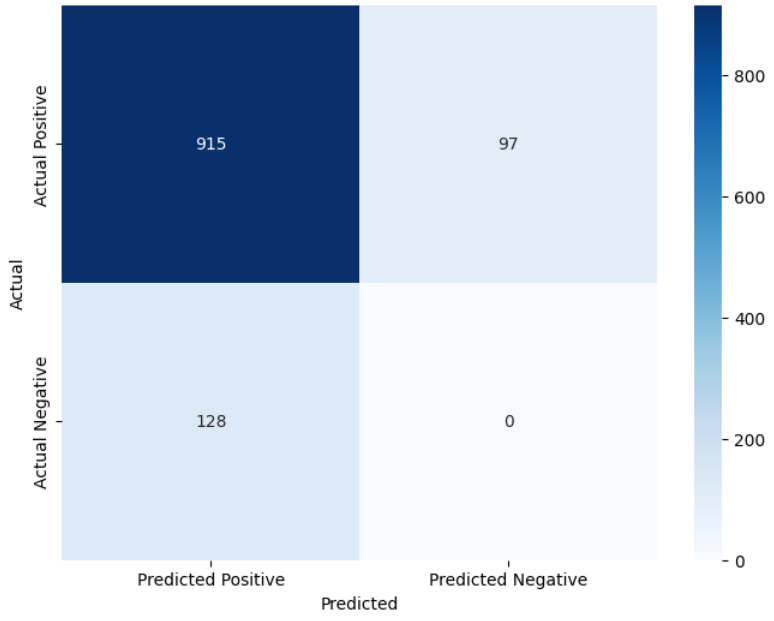
\includegraphics[width=0.5\textwidth]{Images/Diagrams/confusion_matrix.png}
    \caption{\centering Confusion Matrix}
    \label{fig:confusion_matrix}
\end{figure}

The confusion matrix in Figure \ref{fig:confusion_matrix} displays that the model has detected 915 people correctly, failed to detect 128 people, and incorrectly detected 97 people where there were none. For classification tasks, it is common to have the table show which class the model has detected, and which class the object actually is. For single class object detection, the confusion matrix is sufficient as-is.

Further the TPs, FNs and FPs are used to calculate the precision, recall and F1 score of a machine learning model.

\paragraph{Understanding Precision and Recall}
\phantomsection
\label{sec:understandingprecision}
For a balanced metric of precision and recall we also have the F1 Score, combining the two in a single value. Here’s a breakdown of each:

Precision: Measures the accuracy of positive predictions. It is the ratio of correctly predicted positive observations to the total predicted positives. High precision relates to a low rate of false positives. For object detecion of persons, precision would be how accurate the model is when it claims to detect a person.
\begin{equation}
    \text{Precision} = \frac{TP}{TP + FP}
\end{equation}

Recall (Sensitivity or True Positive Rate): Measures the ability of the model to find all the relevant cases within a dataset. It is the ratio of correctly predicted positive observations to the all observations in actual class. High recall relates to a low rate of false negatives. For object detection of persons, recall would tell us how many of the actual persons in the image the model was able to detect. We must note that since precision does not take false negatives into account, using recall as a performance metric may be vital in the situations where detecting all the persons may be important.
\begin{equation}
    \text{Recall} = \frac{TP}{TP + FN}
\end{equation}

F1 Score: The weighted average of Precision and Recall. This score takes both false positives and false negatives into account. It is particularly useful when the class distribution is uneven. F1 Score is best if there is some sort of balance between Precision and Recall in the system.
\begin{equation}
    \text{F1 Score} = 2 \times \frac{\text{Precision} \times \text{Recall}}{\text{Precision} + \text{Recall}}
\end{equation}

The precision-recall curve is commonly used to assess the performance of a general machine learning model (see Figure \ref{fig:precisionrecallcurveexample} for an example). The precision-recall curve is a graph that shows the trade-off between precision and recall for different thresholds for confidence in the object class. As you allow your model to be more uncertain in its inferences\footnote{For object detection, there are at least three ways of allowing the model to be more uncertain. Fixing the confidence threshold and vary the IoU, or fixing the IoU and vary the confidence threshold, or by averaging over both thresholds.}, the number of hallucinations will also increase and thus the precision drops. The area under this curve is the average precision (AP) of the model.

\begin{figure}[H]
    \centering
    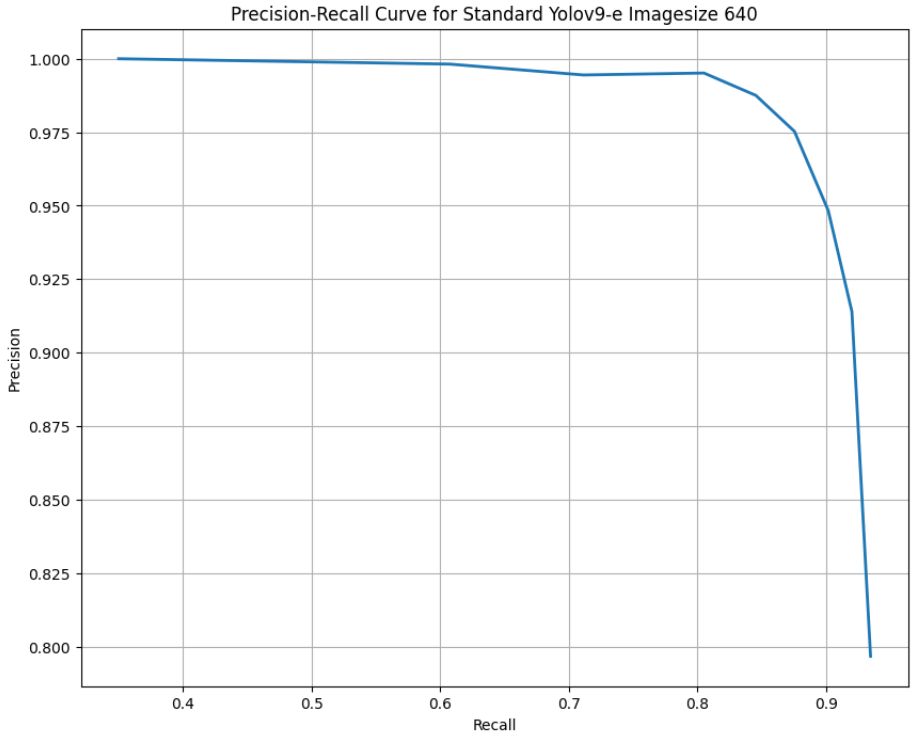
\includegraphics[width=0.7\linewidth]{Images/Results/PR-curve standard e 640.png}
    \caption{\centering Precision-Recall Curve}
    \label{fig:precisionrecallcurveexample}
\end{figure}

The area under the Precision-Recall curve is the average precision (AP) of the model. This can be expressed as follows:
\begin{equation}
    \text{AP} = \sum_{n} (R_n - R_{n-1}) P_n
\end{equation}
where $R_n$ is the recall at the $n$ n-th threshold, $R_{n-1}$ is the recall at the previous threshold, and $P_n$ is the precision at the $n$ n-th threshold.

Alternatively, AP can be represented as an integral:
\begin{equation}
    \text{AP} = \int_{0}^{1} P(R) dR
\end{equation}
where $P(R)$ is the precision as a function of recall $R$.


\paragraph{Understanding the IoU Metric}

Accuracy in object detection refers to both detecting the object \textit{and} its location accurately. Combining both in one metric would simplify benchmarking. The precision, recall and f1-score all neglect the positioning precision of bounding boxes.

For assessing localization accuracy, the Intersection over Union (IoU) is calculated. This compares the predicted bounding box and the ground truth bounding box in a way so boxes need to fit as closely to the ground truth bounding box as possible to get the best score (which is 1.0). See Figure \ref{fig:IoU}. 

\begin{figure}[H]
    \centering
    \begin{subfigure}{0.32\textwidth}
        \centering
        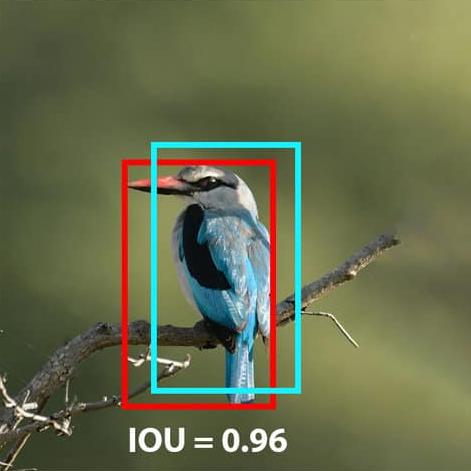
\includegraphics[width=\textwidth]{Images/iou_left.png}
        \caption{\centering True Positive}
    \end{subfigure}
    \hfill
    \begin{subfigure}{0.32\textwidth}
        \centering
        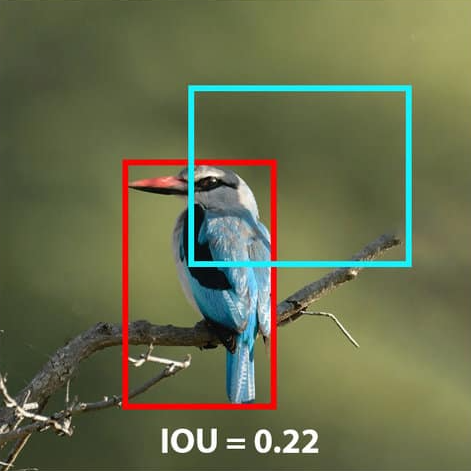
\includegraphics[width=\textwidth]{Images/iou_middle.png}
        \caption{\centering False Positive}
    \end{subfigure}
    \hfill
    \begin{subfigure}{0.32\textwidth}
        \centering
        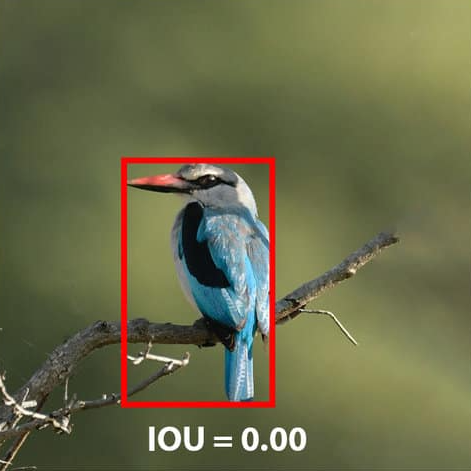
\includegraphics[width=\textwidth]{Images/iou_right.png}
        \caption{\centering False Negative}
    \end{subfigure}
    \centering
    \caption[Intersection over Union (IoU) (\cite{learnopencv_iou})]{\centering Intersection over Union (IoU) (\cite{learnopencv_iou}). The red boxes are the ground truth, and the blue are the model predictions.}
    \label{fig:IoU}
\end{figure}

A high IoU values equates to having a good fit with the ground truth bounding box. If the IoU value is over a certain threshold, we define the detection to be a true positive (see \ref{fig:IoU}a). If the predicted bounding box has little overlap, we identify this as a false positive (see \ref{fig:IoU}b). This may also be called a hallucination. If we don't have detections for a ground truth bounding box (see \ref{fig:IoU}c), we have a false negative. A fourth case is where the predicted bounding box fully overlaps with the ground truth, but covers a larger area. In this case, we have a low IoU due to the high area of union, and thus a false positive. 

The equation for calculating the IoU of a predicted bounding box and a ground truth bounding box is as follows:

\begin{equation}
    \text{Intersect over Union} = \frac{\text{Area of Overlap}}{\text{Area of Union}}
\end{equation}

\paragraph{Conclusion of Performance Metrics}
The Pascal Visual Object Challenge (VOC) was a standard way of measuring performance. Here, the IoU value was fixed (typically at 0.5), while the confidence in detections was averaged over multiple confidence thresholds. The fixed IoU threshold is typically set at 0.5 or higher. Which value is best dependends on the accuracy demands of the sceneario, and is why retaining the ability to adjust the threshold is a good idea when implementing an object detector. Today, the VOC AP metric is seldom used (see \ref{fig:coco_voc_usage}). Following the introduction of MS-COCO datasets in 2014, researchers started to pay more attention to the accuracy of object localization instead of using a fixed IoU threshold (\cite{zou2023object_detection_in_20_years}).

\begin{figure}[H]
    \centering
    \begin{subfigure}{0.40\textwidth}
        \centering
        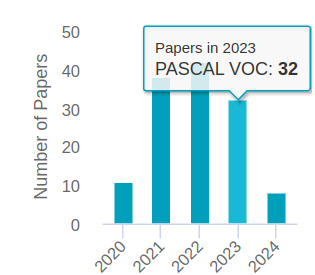
\includegraphics[width=\textwidth]{Images/Dataset Usages/PASCAL.png}
        \caption{\centering Pascal VOC: 32 (2023)}
    \end{subfigure}
    \begin{subfigure}{0.40\textwidth}
        \centering
        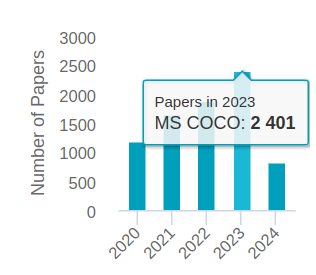
\includegraphics[width=\textwidth]{Images/Dataset Usages/COCO.png}
        \caption{\centering COCO: 2401 (2023)}
    \end{subfigure}
    \caption{\centering PASCAL VOC and COCO Approximate Number of Usages (\cite{papers2024COCOusage})}
    \label{fig:coco_voc_usage}
\end{figure}

The single-most important metric for object detection in the COCO dataset challenge was the mean Average Precision (mAP) over 10 IoU thresholds of .50:.05:.95. This rewards the detectors with more accurate localization (\cite{li2014cocodataset}).

A third method of measuring AP would be to vary both the confidence threshold and the IoU threshold. This would consider both the classification \textit{and} localization accuracy, but the calculation is also computationally heavier. In the Project Results, we discuss whether this computational expense makes a difference in the evaluation of the object detectors in this project on the FIMUS dataset.

\subsection{Object Detection Algorithms}
\label{sec:object_detection}
This subsection includes a brief summarization of the evolution of object detection, including the transition from traditional methods to morw modern methods such as the YOLO series and vision transformers.

The evolution of object detection can be divided into two major historical phases: before and after 2014, as illustrated in Figure \ref{fig:object_detect_20_years}. Prior to 2014, traditional object detection methods, such as the Viola-Jones detectors (\cite{vi2001viola-jones-orig}), Histogram of Oriented Gradients (HOG), and Deformable Part-Based Models (DPMs) were prevalent\footnote{These are just some honorable mentiones of some of the most sucessful and widely adopted models of the time (\cite{li2012violajonessuccessful})}. During this era, \textit{mixture models} were developed to improve detection granularity by recognizing the different parts of the same object, such as the doors and windows of a car.

\begin{figure}[H]
    \centering
    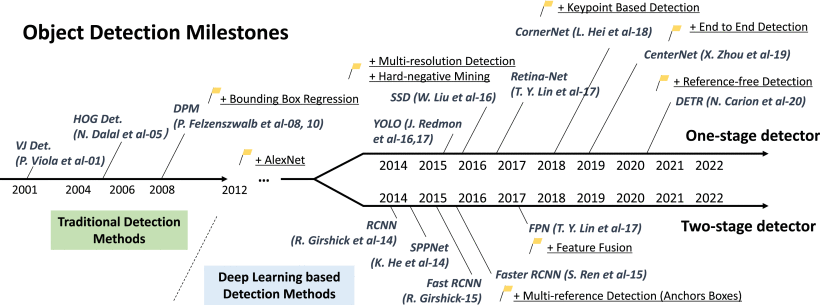
\includegraphics[width=1\linewidth]{Images/Diagrams/object_detection_20years.png}
    \caption{\centering Object Detection Milestones (\cite{zou2023object_detection_in_20_years})}
    \label{fig:object_detect_20_years}
\end{figure}

Despite these advancements, it was not until the introduction of Region-based Convolutional Neural Networks (R-CNN) in 2014 that the accuracy of object detection systems began to improve significantly. This paradigm shift marked a substantial advancement in the field, leveraging deep learning techniques to enhance detection performance dramatically (\cite{zou2023object_detection_in_20_years}). The period following 2014 has seen rapid progress, introducing sophisticated object detectors like You Only Look Once (YOLO) and Detection Transformers (DETR). 

\newpage
\subsubsection{You Only Look Once (YOLO)}
\label{sec:yolo}
The YOLO (You Only Look Once) object detection algorithm is renowned for its efficiency in real-time object detection. YOLO divides the image into a grid and predicts bounding boxes and class probabilities for each grid cell. Unlike traditional object detection algorithms that require multiple passes through a network, YOLO processes images in a single pass. This approach significantly enhances detection speed. The YOLO algorithm was the first one-stage (single pass) detector, and led the way for the development of other various popular networks such as the RetinaNet and DETR.

\paragraph{YOLOv3}
YOLOv3 marked a significant advancement in the YOLO series by integrating multi-scale predictions and a deeper feature extractor. A deeper feature extractor refers to the use of more layers in the convolutional neural network (CNN), which allows the model to capture more complex features from the images. These improvements improved speed and accuracy from the first versions of YOLO.  

\paragraph{YOLOv9}
YOLOv9 represents what was the latest and most advanced version in the YOLO series at the beginning of this thesis project. It features numerous optimizations for faster training and increased accuracy, especially in challenging conditions such as low light and occlusions. YOLOv9's architecture is streamlined to reduce computational overhead, enabling it to perform well even on less powerful devices. This version also benefits from enhanced post-processing techniques that refine the accuracy of its predictions.

\paragraph{YOLOv10}
YOLOv10, built with ultralytics and RT-DETR, is the current latest addition to the series. The commit message "add yolov10" was made on 23rd of May, signalling the first date of the release.

\subsubsection{Detection Transformers (DETR)}
\label{sec:detr}
The Detection Transformer (DETR) is an innovative machine learning method introduced by the Facebook (Meta) Research team. DETR leverages a transformer encoder-decoder architecture, similar to those used in natural language processing models. This architecture enables the model to handle complex object detection tasks by processing global information within images, rather than relying solely on local features. See Figure \ref{fig:detrarchitecture} for an illustration of the architecture.

\begin{figure}[H]
\centering
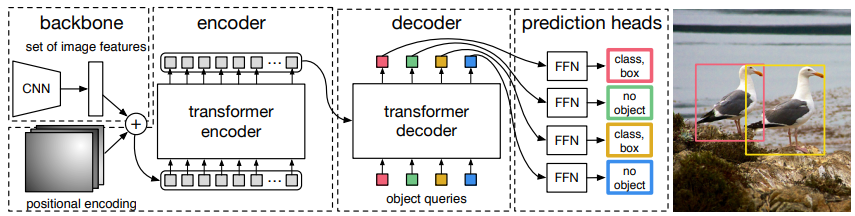
\includegraphics[width=1\linewidth]{Images/Diagrams/DETR2.png}
\caption{\centering The Architecture of the DETR Model (\cite{carion2020endtoend})}
\label{fig:detrarchitecture}
\end{figure}

In the paper where DETR was first introduced, \citeauthor{carion2020endtoend} demonstrated that DETR outperforms several competitive baselines on tasks such as panoptic segmentation\footnote{This is a challenging pixel-level segmentation task where an image is divided into meaningful regions.}. They achieved these results by integrating a simple segmentation head trained on top of a pre-trained DETR.

\newpage
The conclusions of their study highlight the potential of DETR:

\begin{myquote}
    We presented DETR, a new design for object detection systems based on transformers and bipartite matching loss for direct set prediction. The approach achieves comparable results to an optimized Faster R-CNN baseline on the challenging COCO dataset. DETR is straightforward to implement and has a flexible architecture that is easily extensible to panoptic segmentation, with competitive results. In addition, it achieves significantly better performance on large objects than Faster R-CNN, likely thanks to the processing of global information performed by the self-attention. This new design for detectors also comes with new challenges, particularly regarding training, optimization, and performances on small objects. Current detectors required several years of improvements to cope with similar issues, and we expect future work to successfully address them for DETR. (\cite{carion2020endtoend})
\end{myquote}

The conclusions encapsulates the core innovations and findings of the DETR model. However, the authors also acknowledge the challenges that come with this new approach. Training and optimizing DETR is complex, especially when dealing with small objects. The initial performance issues on training and optimalization present challenges in terms of being able to fine-tune the models to a specialized dataset. Despite these challenges, the authors express optimism that DETR can overcome these initial hurdles, much like how earlier detectors evolved over time. 

\subsubsection{Comparison of YOLO and DETR}

While DETR offers a groundbreaking approach by utilizing transformers for object detection, its complexity and the need for domain-specific training models can limit its adaptability and scalability. In contrast, the YOLO series, particularly YOLOv9, provides a more robust solution for real-time applications. YOLO's ability to quickly process images, coupled with continual improvements in both speed and accuracy, makes it a more practical choice for diverse and dynamic environments.

The introduction of YOLOv9 highlights a notable weakness in the DETR series. \citeauthor{wang2024yolov9} pointed out:

\textit{However, since it is extremely difficult for DETR series object detector to be applied to new domains without a corresponding domain pre-trained model, the most widely used real-time object detector at present is still YOLO series.} (\citeyear{wang2024yolov9})

This assessment underscores the flexibility and widespread adoption of the YOLO architecture in various operational contexts. In contrast, DETR's specialized and computationally intensive requirements make it less versatile for broader applications without significant adjustments and domain-specific training. Thus, while DETR presents a novel and highly effective approach, YOLO remains the preferred choice for real-time, adaptable object detection tasks.

\subsubsection{Dark-Lit Environments}
Being able to detect and locate people in dark-lit environments have been previously attempted, usually for security concerns in public spaces. \citeauthor{pa2020PersonDetectionNightTimeFLIR} developed a system for detecting people in dark-lit environments using a convolutional neural network (\citeyear{pa2020PersonDetectionNightTimeFLIR}). They modified the three input channels which usually take RGB to take as input instead (i) the original infrared image, (ii) a difference image from the previous frame, and (iii) a background subtraction mask. Their dataset is vastly different from the setting for this thesis, as the individuals in their photos were far away from the cameras. However, they found that their system was able to detect people in dark-lit environments with an accuracy of 90\%. This is a promising result, as it shows that it is possible to detect people in dark-lit environments using infrared imaging and CNNs. They used FLIR cameras, which make images from heat. Doing inferences on pure infrared images may be harder because the infrared radiation may be less prevalent than the heat a FLIR camera may capture. The FLIR cameras are expensive, and thus not considered viable for this project.

The article "YOLO in the Dark - Domain Adaptation Method for Merging Multiple Models" by \citeauthor{Sasagawa2020YOLO} presents a novel approach for improving object detection in low-light conditions (\citeyear{Sasagawa2020YOLO}). 

The key facets and findings were: 
\begin{itemize}
    \item The proposed method merges pre-trained models from different domains using glue layers and a generative model, enabling adaptation to new tasks without additional datasets. 
    \item The YOLO-in-the-Dark model combines the "Learning-to-See-in-the-Dark" model with the YOLO model, enhancing object detection capabilities in low-light images. 
    \item By creating latent features from existing datasets, the generative model trains glue layers efficiently, reducing the need for new data and computational resources. 
    \item The YOLO-in-the-Dark model effectively detects objects in raw short-exposure low-light images with fewer computing resources than traditional methods.
\end{itemize}

These findings highlight the model's potential for efficient, high-performance object detection in challenging lighting conditions, making it a valuable tool for person localization applications in real-world low-lit environments.

\subsubsection{Transfer Learning and the Effectiveness of Fine-tuning}
\label{sec:transfer_learning_fine_tuning}
Transfer learning is the process of transferring knowledge from a source domain to a different but related target domain. In practice, this means having a pre-trained model fine-tune on a dataset that is specialized for the task at hand. Extending a model's capabilities to learn to correctly identify a new object class or improving the detection accuracy are typical examples of transfer learning use cases. The following research on transfer learning for object detection models demonstrates accuracy gains when fine-tuning pre-trained models compared to training from scratch. 

\citeauthor{Wei2024FeatureCorrective} introduced Feature Corrective Transfer Learning (FCTL) in their study (\citeyear{Wei2024FeatureCorrective}). This approach enhances object detection in non-ideal visual conditions by incorporating a feature similarity loss during training. The Non-Ideal Image Transfer Faster R-CNN (NITF-RCNN) model, developed using this method, showed improved detection accuracy in challenging environments by aligning feature maps between ideal and non-ideal images.

Another study used a generative model to create synthetic training data, which was then used to pre-train an object detector (\cite{TransferLearningGenerative2023}). This pre-trained detector was subsequently fine-tuned on a limited real dataset. This method, applied to detect cars in urban environments and fish in underwater settings, resulted in improved detection accuracy compared to using real data alone. The key advantage was leveraging the large synthetic dataset to enhance the detector's initial training phase before fine-tuning it on the actual data, yielding better performance in both domains. An illustration of the process is depicted in figure \ref{fig:training_data_generated}.

\begin{figure}[H]
    \centering
    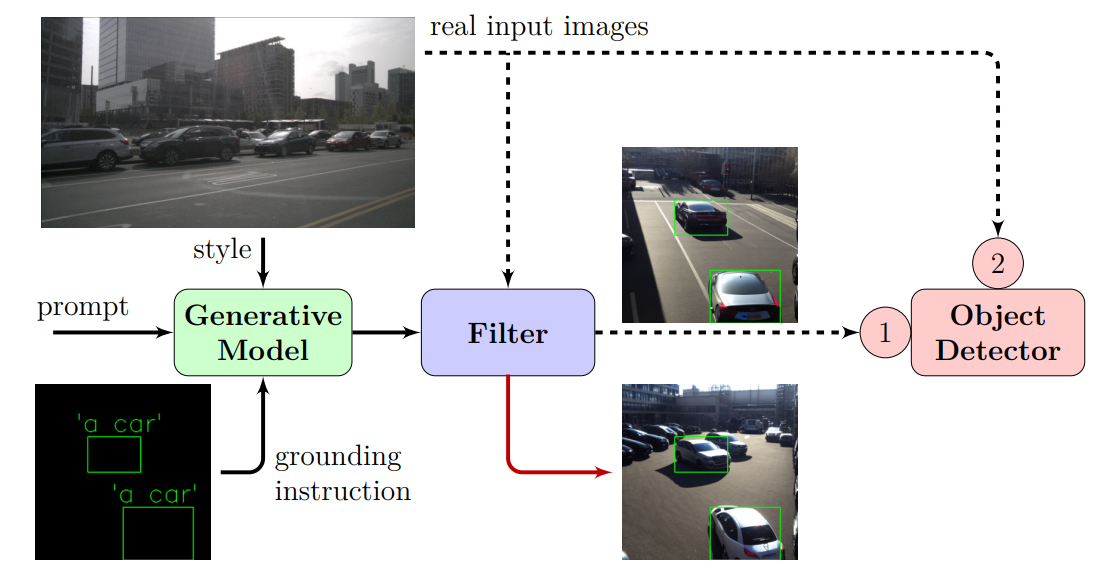
\includegraphics[width=\textwidth]{Images/Diagrams/generated_training_images.png}
    \caption{Transfer Learning for Object Detection With Generative Models (\cite{TransferLearningGenerative2023})}
    \label{fig:training_data_generated}
\end{figure}

Description for Figure \ref{fig:training_data_generated} as given by the authors:

\begin{myquote}
    We employ a L2I pretrained model to generate images for transfer learning to an object detector. We can filter out suboptimal generated images based on benchmark metrics. For instance, the image along the red arrow is discarded because the generative model has depicted many cars outside the bounding boxes designated in the grounding instruction. With the remaining generated images, we pretrain the object detector, followed by a fine-tuning on the real dataset. Dashed lines indicate the data used for training the models. (\cite{TransferLearningGenerative2023})
\end{myquote}

Generating artificial training data is not uncommon practice for model fine-tuning. \citeauthor{el2017WTB} discussed some of the challenges with visual systems in an investigation of an existing internet of things (IoT) system for wildlife monitoring \textit{Where's The Bear}. The system suffered from three major drawbacks; (1) the transmission of enormous numbers (sometimes millions) of images over low-bandwidth networks, which tend to happen in automatically (motion-) triggered applications, (2) motion sensors triggered by weather conditions or by animals that were not of interest, and (3) redundancy of images taken of the same individual animal.

\citeauthor{el2017WTB} implemented solutions to the challenges. The first solution was to utilize edge computing to avoid sending every image online. This is an approach to achieve low-latency, high bandwidth, high availability, low cost communications and fast response to/from the sensors. In this thesis we make the distinction between edge computing and on-device processing. Edge computing is when the processing happens \textit{close to} the edge, but not necessarily on the device itself. For \textit{Where's the Bear's} solution, the data was transmitted to a device close to the sensors for processing, greatly reducing the distance for the transmissions. 

The next solution of \citeauthor{el2017WTB}, was to train their models using artificially produced, specialized training data. Since images of bears are uncommon and they needed a high number of images of bears, they took empty images from the wildlife camera's and placed them in images to improve the model. See figure \ref{fig:wtb_bears}.

\begin{figure}[H]
    \centering
    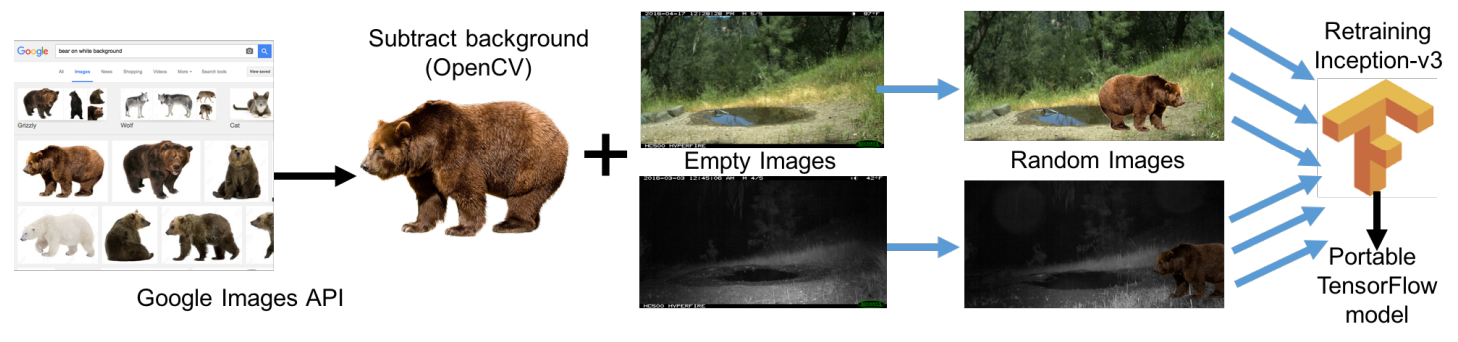
\includegraphics[width=\linewidth]{Images/artificial_bears.png}
    \caption{Where's the Bear's Artificially Placed Bears (\cite{el2017WTB})} 
    \label{fig:wtb_bears}
\end{figure}

The results of the study was, however, that a model trained on real images from one of the cameras performed slightly better than the one trained on artificially produced images. This motivates the decision to not put artificially placed humans in images for a person localization system. 

The results of these aforementioned studies show that accuracies of machine learning models may be improved by fine-tuning on specialized data. Next, the thesis outlines some third-party services and products, similar to the Where's the Bear system, that were included in this thesis for their possible usefullness to the project.

\subsection{Third-Party Services}
\label{sec:thirdparty}
Roboflow is a platform designed to simplify and enhance the process of building and deploying machine learning models, particularly in the domain of computer vision. The platform offers comprehensive tools for data management, model training, and deployment, making it highly valuable for applications requiring precise object detection, including the localization and detection of persons.

\subsubsection{Roboflow}
Roboflow's ecosystem comprises several key components that streamline the development of computer vision models:
\begin{itemize}
    \item \textbf{Data Management}: Roboflow provides tools for annotating, organizing, and augmenting image data. These features facilitate the creation of high-quality datasets that are essential for training accurate models. Datasets created with these tools are then stored and hosted on the Roboflow server, open for other people to use.
    \item \textbf{Pre-Trained Models}: The platform offers a wide range of pre-trained models optimized for various tasks. Users can leverage these models to accelerate the development process, especially when combined with transfer learning techniques to adapt these models to specific tasks. This also means that any model you create yourself will be available for your potential industry competitors.
    \item \textbf{Model Training and AutoML}: For users without deep technical expertise in model architecture, Roboflow's AutoML capabilities offer an automated way to generate models tailored to their unique datasets. This enables a quick and easy-to-grasp way of implementing machine learning for a use case.
    \item \textbf{Deployment}: Roboflow enables seamless model deployment via APIs, allowing models to be integrated into applications effortlessly. This API-driven approach supports both cloud-based and local deployments, ensuring flexibility according to user needs with regards to inference speed due to network latency and data privacy and security.
\end{itemize}

The platform's ability to manage and process data through a user-friendly interface allows for rapid iteration and experimentation, reducing the time from concept to deployment.

\textbf{Use Case: Detection of Persons}

Roboflow excels in scenarios requiring the detection of specific objects within varied environments, such as detecting persons in crowded or complex scenes. The platform supports the deployment of models capable of identifying and localizing persons with high accuracy, which is crucial for applications in security, retail analytics, and urban planning.

One application would be using Roboflow to train models on the CrowdHuman dataset, without the need to download the dataset or train the model locally. Models may be fine-tuned for scenarios such as monitoring museum traffic. The \href{https://roboflow.com/}{Roboflow website} contains multiple guides for how such applications may be implemented.

\subsubsection{OpenAIs Generative Pretrained Transformer 4 (GPT-4) with Vision}
The capabilities of large language models (LLMs) have expanded beyond text to include various tasks, such as visual processing. GPT-4 with Vision is an example of a multimodal model (LMM). Many products already integrate OpenAI's ChatGPT, and adding visual capabilities can enhance these applications. LLMs with vision can semantically understand scenes, like predicting a riot in a bar street in England or recognizing a fish feeding event at an aquarium, and gauging crowd reactions\footnote{There has been considerable research focused on detecting the mood of people. This requires high resolution images of good quality. One model would detect people or faces, and another would get cut-outs of those faces to detect the mood of each individual.}. This could allow automated applications to provide insights without human analysis, making them faster, more accurate, and scalable compared to current surveillance systems.

However, the generative nature of GPT models poses a challenge: their performance can vary daily. While many experiments show promising results, they are static and may not reflect consistent performance over time. Consequently, models may perform well in tests but fail post-deployment.

To address this, a \href{https://www.gptcheckup.com/}{website} has been dedicated to measure how the GPT-4 with Vision\footnote{Previously called GPT-4V \href{https://platform.openai.com/docs/guides/vision}{https://platform.openai.com/docs/guides/vision}.} performs across a range of experiments. The website is made by the team at Roboflow, but let's other users submit their experiments for daily checkups through git pull requests. Out of 13 of the experiments currently posted, 5 have failed every day the last 7 days, and 2 have failed at least once in the last 7 days. One of the experiments, counting fruits in a bowl, is alternating every day between success and failure. This proves the point that generative models may still be considered too unreliable for many applications.

Further, in May 2024, OpenAI introduced its newest edition of the renounced ChatGPT series; the ChatGPT-4o. \textit{o} is for omnimodal, and refers to its ability to perform in a multitude of modalities, including vision. This model was tested for the task of object detection, but rendered unsatisfactory performances\footnote{The other GPT models \textit{Gemini}, \textit{GPT-4 with Vision}, and \textit{Claude 3 Opus} were previously tested for the identical task, and failed.}. A review of ChatGPT-4o, including a more in-depth description of the experiment on object detection, is found \href{https://blog.roboflow.com/gpt-4o-vision-use-cases/}{here}. The experiment is displayed in Figure \ref{fig:gpt4o_experiment}. ChatGPT-4o, misplaced two bounding boxes when prompted to detect the dog in the image.

\begin{figure}[H]
    \centering
    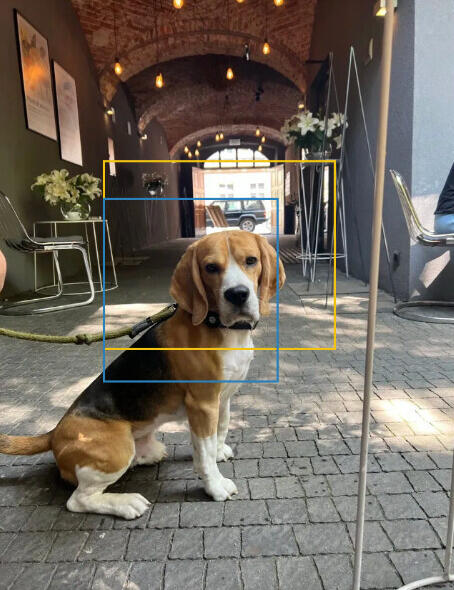
\includegraphics[width=0.4\textwidth]{Images/gpt4o_object_detection_just_dog.jpg}
    \caption{\centering ChatGPT-4o Object Detection Experiment (\cite{ue2024chatgpt4o})}
    \label{fig:gpt4o_experiment}
\end{figure}

The two preceding sections highlights the strengths and capabilities of third-party services such as Roboflow and GPT4-V, but there are some more downsides not yet mentioned that need to be evaluated before moving forward with a third-party option. Further discussion of third-party services are found in Section \ref{sec:discuss_thirdparty}.

\subsection{Third-Party Products}
\label{sec:thirdparty_products}
Intelligent visual edge image/video devices seem to have an endless number of applications. In the following section we will take a look at some actors and their products to get an overview of the market of edge AI cameras.

The target of products such as the 'EufyCam 3' and the 'Aqara FP2 mmWave' is the private smart home sector. The i-PRO's WV-S71300-F3 has many of the same functionalities but targets enterprises instead. These products are presented in the following paragraphs and displayed in Figure \ref{fig:solutions_on_the_market}.

\subsubsection{EufyCam 3}
\label{sec:eufycam}
The EufyCam 3 is a battery driven camera with solar a panel, only requiring two hours of sunlight to become fully charged. The EufyCam has functionality for face recognition. This is a self-learning AI which improves with time, up to an accuracy of 99.9\% \cite{eufycam}. To do this, the cameras communicate to an edge computing 'home base' to perform the machine learning tasks, and to save images to a hard drive. You may see an image of the EufyCam product in Figure \ref{fig:eufycam_3}.

The EufyCam deals with low light situations in two different ways: a motion activated spotlight, turning on to film in the dark with a self-provided source of light, and a black and white night vision using six infrared LEDs to capture the video. There's also functionality to set activity areas, and to detect animals or cars.

Eufy's product does not assure privacy by deleting or obscuring images, but rather keeps them on the local area network (LAN). The user's privacy is preserved through storing the videos and images on a private in-house 1TB device, communicated from the camera devices via 2.4GHz WiFi.

The EufyCam 3 product is an edge computing device, and the Prasidh Chhadbria, director of Harvard Undergraduate AI, highlight three main advantages of the edge computing approach (\citeyear{ch2022youtube_edge_computing_eufycam}). (1) Time saved, as the edge devices do not have to constantly send a lot of data to the cloud; (2) Save on cost in terms of cheaper local storage, rather than more expensive cloud storage; (3) Privacy. The data is not sent to another server, but exists on the device itself so you have more control over where your data is going.

\subsubsection{Aqara Presence Sensor FP2}
The Aqara FP2 utilizes multiple passive infrared (PIR) sensors rather than a RGB camera to make detections. The FP2 may detect falls, and can localize up to 5 persons in an area, but a device may only do one of the functionalities at a time. This is due to the fact that fall detection requires the device to be mounted in the ceiling, while presence detections are only accurate when the device is mounted on the wall.

However, the devices has more functionalities. With the ability to set rules for separate zones in the area, one may toggle lights only where a person is located, for example over a workbench. Making this application part of a visual system would possibly facilitate for more applications such as being able to automatically label specific items in the area. One could combine the use of zones with a visual computing module where it would only compute and analyze data, not only when something in the frame is moving (which is typical for wildlife detection cameras (\ref{sec:deletion_of_images})), but when certain rules are triggered, such that a person has been located in a certain zone for a specified amount of time.

\subsubsection{i-PRO}
Another big actor is i-PRO, providing AI network cameras to the market with edge computed people counting, face detection, and people attribute search
(See their product: \href{https://i-pro.com/products_and_solutions/en/surveillance/products/wv-s71300-f3}{product wv-s71300-f3}). The applications of the cameras they offer are often video monitoring and security features. i-PRO has informational web pages about surveillance policies and security. Most, if not all, of their cameras are NDAA compliant as well, which is a requirement to use them on american federal ground with regards to who produces the hardware of the system. Trusted manufacturers is a requirement for products capable of breaching privacy. See \href{https://i-pro.com/}{i-PRO's website} for more information.

i-PRO had a big project where over a 100 cameras were installed in a arts museum in Monaco, where their cameras AI VMD that will give intrusion alerts when movement is detected in areas that should not be accessed, and virtual line crossing, giving alerts when people have crossed a digitally set line of an image. They also had AI scene change detection, detecting any changes in the image in a fixed part of the scenery. Also, AI people detection was used so to generate details about the visitors, so that guards that were interested in specific individuals had to opportunity to track specific individuals. These applications also generated statistics so the costumer had an overview of knowing in real time how many visitors were in the museum and even in the separate rooms or in front of each gallery. The cameras used in this solution were all fish-eye models, illustrating how fish-eye lenses may be the way to go for inside-application areas.

\begin{figure}[H]
    \centering
    \begin{subfigure}{0.2\textwidth}
        \centering
        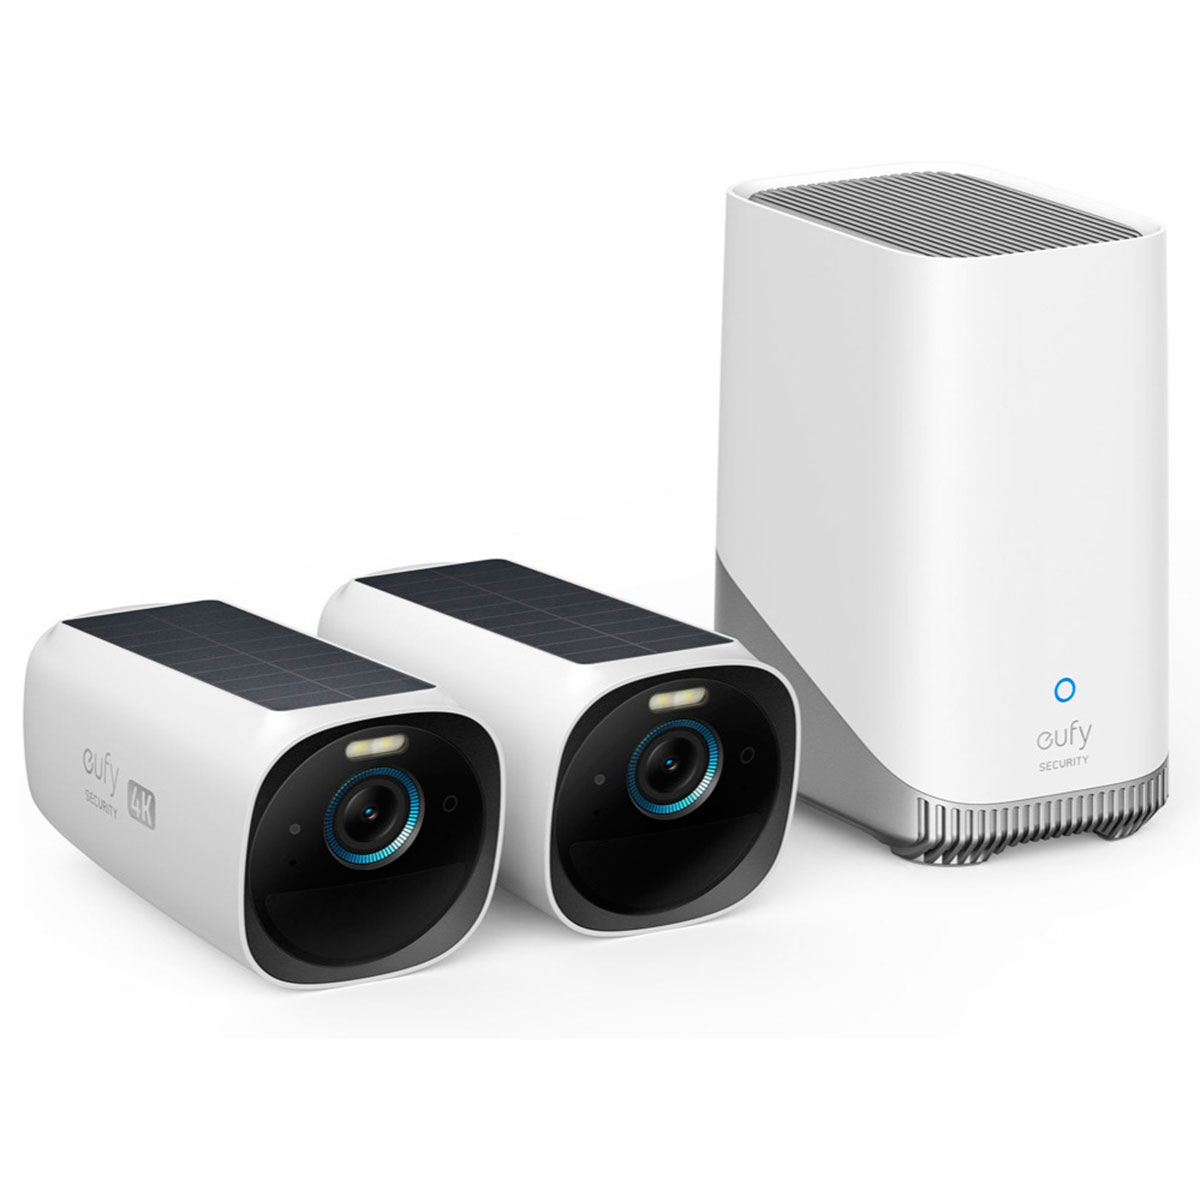
\includegraphics[width=\textwidth]{Images/Products/eufycam3.jpg}
        \caption{\centering EufyCam 3}
        \label{fig:eufycam_3}
    \end{subfigure}
    \hspace{30pt}%
    \begin{subfigure}{0.2\textwidth}
        \centering
        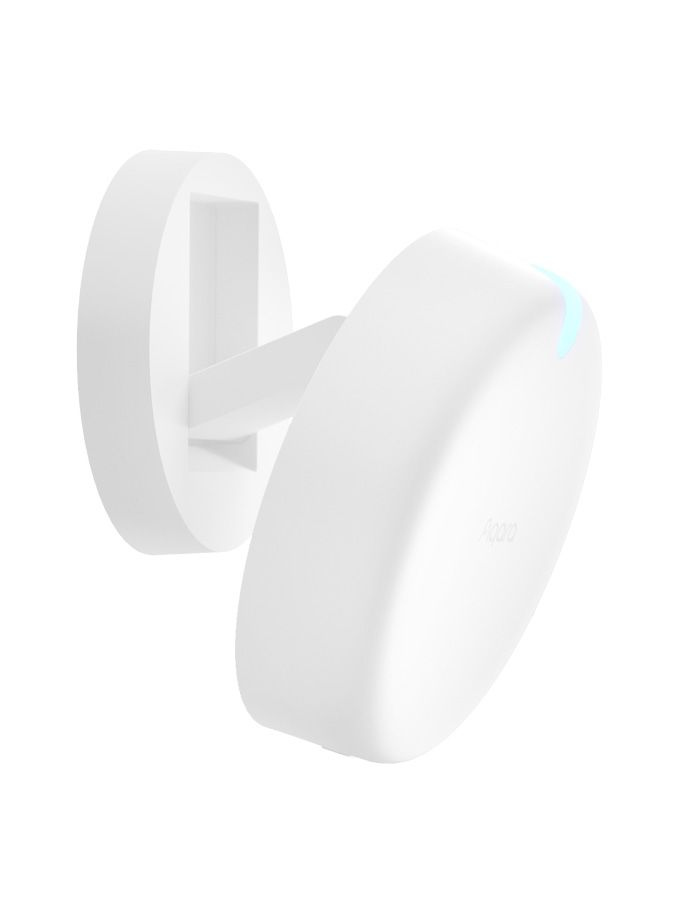
\includegraphics[width=\textwidth]{Images/Products/aquara_fp2.jpg}
        \caption{\centering Aquara FP2}
        \label{fig:aquara_fp2}
    \end{subfigure}
    \hspace{30pt}%
    \begin{subfigure}{0.2\textwidth}
        \centering
        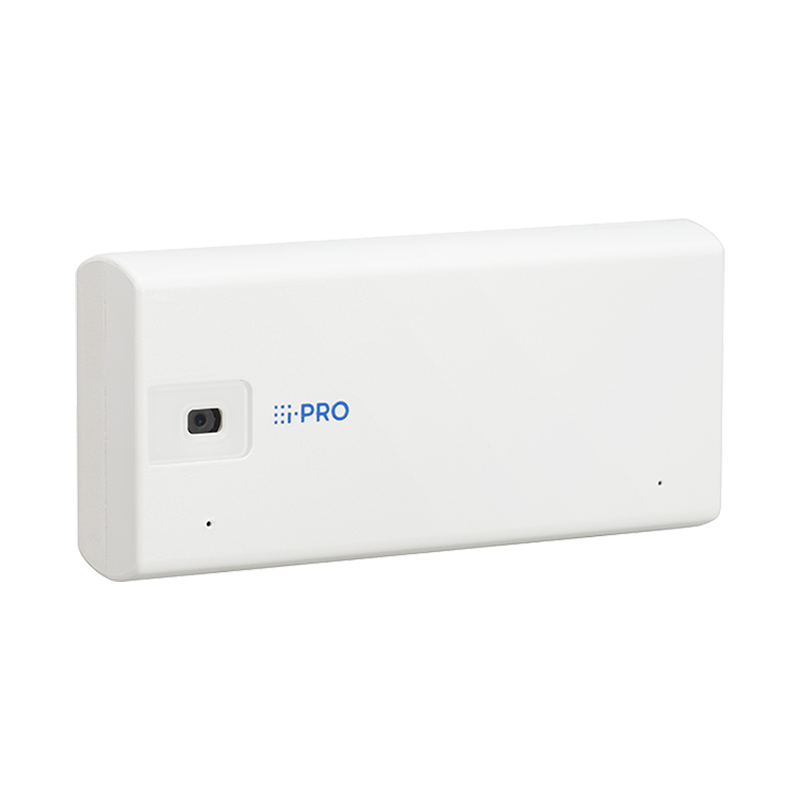
\includegraphics[width=\textwidth]{Images/Products/iPRO_wv-s71300-f3.png}
        \caption{\centering i-PRO WV-S71300-F3}
        \label{fig:i-PRO_camera}
    \end{subfigure}
    \caption{\centering Smart Cameras From Aquara, Eufy and i-PRO}
    \label{fig:solutions_on_the_market}
\end{figure}

\subsubsection{Viso}
\label{sec:viso}
Viso.ai offers products for nearly every use case from abandoned luggage at airports, real time video stream weapon detections, detection of stopped vehicles, to parking space information. Their no-code platform (Viso Suite) enables a fast pipeline for developing new applications out of existing software. Viso.ai also has a lot of great articles on their web page regarding visual computing topics (see for example \cite{bo2023yolov7_guide}). The Viso Suite is marketed as a way to \textit{Automate manual work, reduce development costs, solve scaleability, privacy and security end-to-end, accelerating every step of the enterprise computer vision development life cycle}. (This thesis is not sponsored).

\subsubsection{VMukti}
Not only does VMukti have some of the longest and most confusing product names on the market (\textit{Real-time Edge AI based Smart Cloud Camera}), but also some of the biggest fishes in their pond of costumers. This pond includes Google, Amazon Web Services, and Microsoft\footnote{Also Azure, which is owned by Microsoft}. One of their products, the Real-time Edge AI based Smart Cloud Camera, provides the user with a live stream of video from the camera. This may create privacy issues should the wrong user get access to the video stream, and it is likely demanding more power and network bandwidth than what it would take to only communicate the results of an analysis. VMukti's other product, the \textit{Edge AI Based 5MP PTZ ANPR Bullet Camera VM-72BPTZ5AIVE} is listed with cutting edge technologies, including \textit{local data processing, filtered data transfer to the cloud, and faster decision-making}. However, its hard to figure out from their website what data is processed locally, and what their decision-making is faster than.

VMukti delivers solutions for surveillance of vehicles, school buses, healthcare, shopping malls, smart cities, warehouses, campuses, examinations, premises, elections and banking. For outside monitoring, VMukti offer cameras that may connect through the mobile network, for monitoring outside remote locations.

\subsection{Hardware}
\label{sec:hardware_options}
Both single board computers and microcontrollers are viable options for devices capable of on-device processing. In this section, we present some considerations regarding microcontrollers, followed by a brief presentation of three single board computers; the Raspberry Pi 3 model A+, the NVIDIA Jetson Nano, and the Radxa/OKdo ROCK 4 SE

\subsubsection{Microcontrollers}
A microcontroller differs from a single-board computer in that it lacks the general-purpose user interface and memory management functionality that a more general-purpose computer would have. A microcontroller is basically just a chip, and are generally supposed to run one task repeatedly. Some options for microcontrollers are the ESP32 or the MAX78002. The latter is optimized for convolutional neural net operations, which would speed up the inference latency. This would most likely be a great option for a person localization system. 

A microcontroller must be programmed. eCos, short for "Embedded Configurable Operating System," presents a compelling alternative for microcontroller applications. Unlike traditional, general-purpose operating systems like Ubuntu or Debian designed for desktop or server environments, eCos is specifically tailored for resource-constrained systems. The lightweight and configurable nature makes it well-suited for microcontrollers with limited processing power and memory. eCos provides a modular architecture, allowing developers to selectively include only the components necessary for their particular application, minimizing the overall footprint. This level of customization enables efficient utilization of hardware resources and ensures optimal performance in environments where efficiency is paramount. 

Additionally, eCos is open-source, fostering a collaborative development community (still alive today \href{https://ecos-discuss.ecos.sourceware.narkive.com/IaITkLWC/is-ecos-project-still-alive\#post2}{blog post}), enabling developers to adapt the operating system to the unique requirements of their microcontroller-based projects. Overall, eCos stands out as a viable and adaptable choice for systems where an operating system tailored to the specific demands of microcontroller applications is required.

Another option for an operating system is MicroPython. In an article on \href{realpython.com/micropython}{realpython.com/}, the author includes multiple compatible hardware, for example the ESP8266 and \textbf{ESP32}. MicroPython has its advantages in simplicity, ease of use, and powerful capabilities. 

\subsubsection{Single-Board Computers}
A simpler-to-implement system would use a single-board computer with a general purpose, widely adopted operating system instead. There are multiple options to pick from. The best option depends on the use case sceneario and budget. We present three options for single-board computers able and suitable for person localization systems.

\paragraph{Raspberry Pi}
The Raspberry Pi company has provided single-board computers since 2012 that are beginner-friendly and affordable. They are considered great options for general computing devices, and are popular for novices to get an introduction to edge device programming. The SBCs are also a viable option for applications that do not demand a lot of computational power. Raspberry Pi comes in several models and series, with Raspberry Pi 5 being the newest addition.  

\paragraph{Jetson Nano}
Measuring in GFLOPs (an indirect measure for AI performance), the Jetson Nano board has a nearly 22x performance advantage over the Raspberry Pi model 3. This is reflected in the pricing, as the Jetson Nano is considerably more expensive (149USD on Amazon.com compared to Raspberry Pi at 35USD for single purchases (14 of December, 2023)). The Jetson is developed by NVIDIA, the leading company when it comes to AI and deep learning. NVIDIA is the company behind CUDA, a software toolkit for utilizing GPUs for accelerated processing.

The Jetson Nano Developer Kit has two camera serial interfaces (CSIs), enabling stereo vision. Additionally, it has a 128-core CUDA GPU, making it the computationally strongest out of this selection, and the most fit for running AI applications. However, Jetson Nanos have been hard to source in the past, and are a bit more expensive than the two other SBCs.

\paragraph{ROCK 4 SE}
Another consideration is Radxa and OKdo's\footnote{They seem to have a partnership, making them both the developer and distributors of the ROCK SBCs.} ROCK 4 SE. It is one out of four models in the ROCK 4 series. Entering the market as an alternative to the Raspberry Pi, it includes all the necessary components and interfaces for advanced video and imaging tasks, such as object detection. It also has better performance than the aforementioned single board computers. It does not have any AI-enhancing hardware, however, only a strong CPU which is not what is usually prioritized for AI-specific hardware. The ROCK 4 SE supports USB type C 12V.

There's also the upgraded ROCK 5 model A, featuring both a GPU and a 6TOPS (Tera operations per second) NPU. TOPS is not a good measurement on its own due to the fact of neural networks consisting of more than only the operations which the NPU is specialized to perform. Therefore, having computational strong hardware to back up a high throughput otherwise as well is important for an NPU to be fully utilized; if not, it will only wait for the CPU to finish its mid-inference operations (\cite{ai2021TOPS}).

\begin{figure}[H]
    \begin{subfigure}{0.24\textwidth}
    \centering
        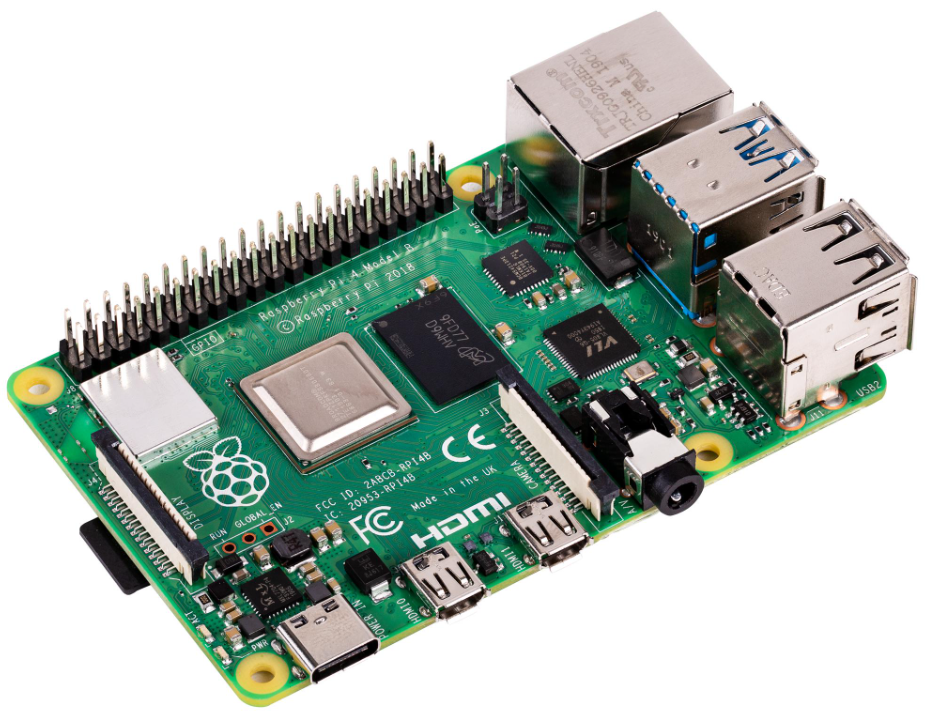
\includegraphics[width=\textwidth]{Images/Hardware/rpi-4b.png}
        \caption{Raspberry Pi 4 model B}
        \label{fig:rasp_pi_3A+}
    \end{subfigure}
    \hfill
    \begin{subfigure}{0.24\textwidth}
        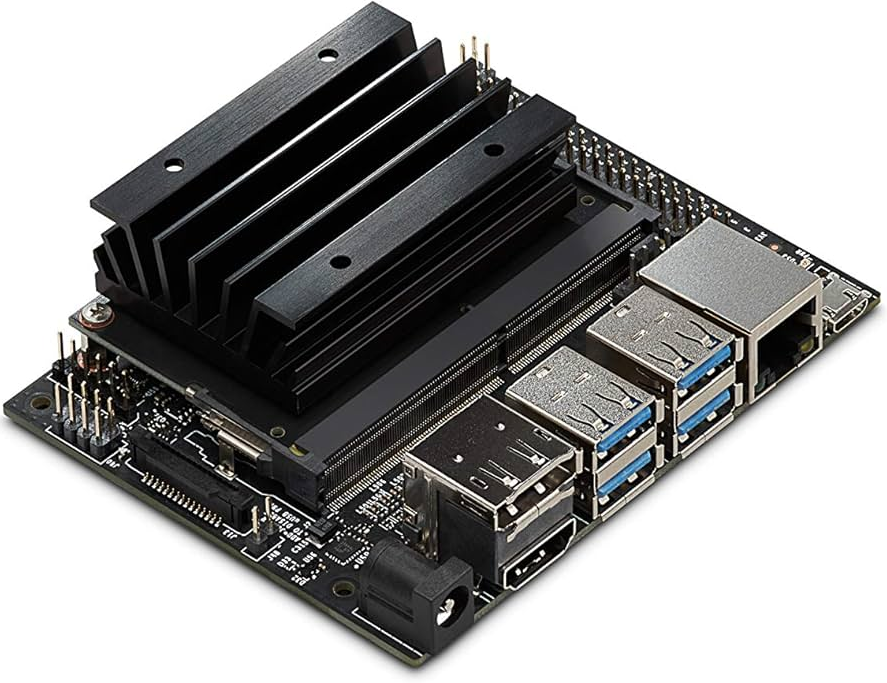
\includegraphics[width=\textwidth]{Images/Hardware/jetsonnano.png}
        \caption{NVIDIA Jetson Nano}
        \label{fig:jetson_nano}
    \end{subfigure}
    \hfill
    \begin{subfigure}{0.24\textwidth}
        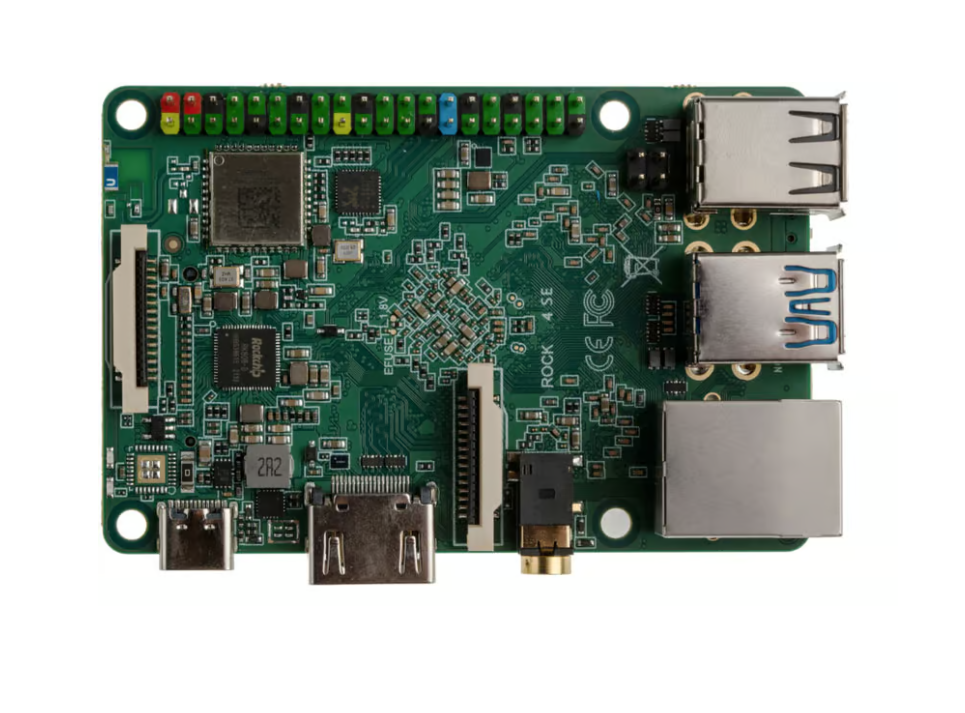
\includegraphics[width=\textwidth]{Images/Hardware/rock4.png}
        \caption{Radxa ROCK 4 SE}
        \label{fig:rock4}
    \end{subfigure}
    \hfill
    \begin{subfigure}{0.24\textwidth}
        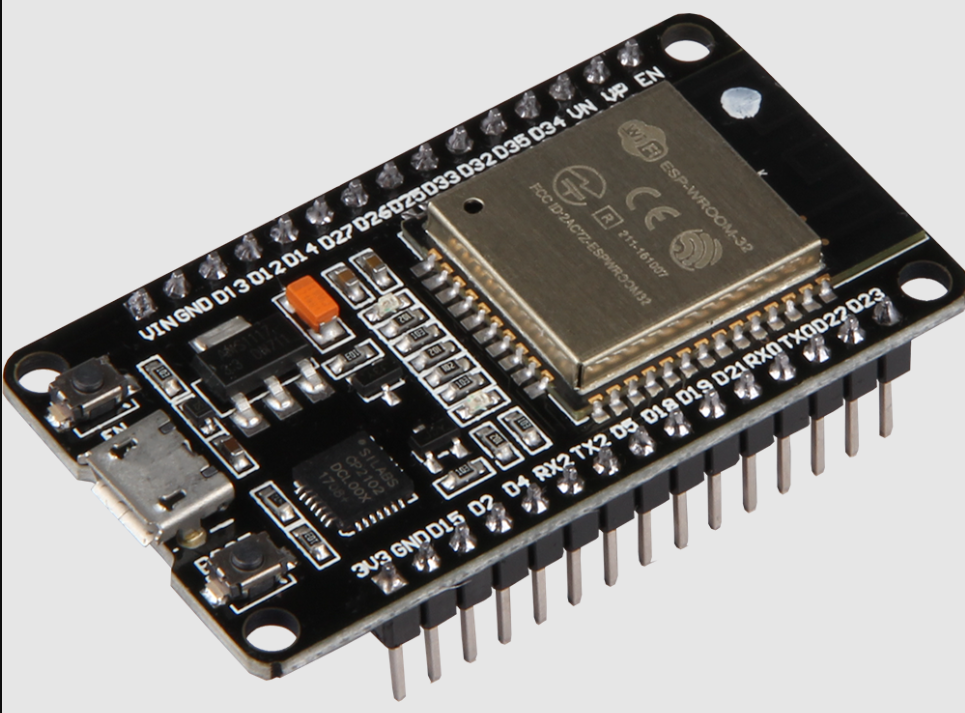
\includegraphics[width=\textwidth]{Images/Hardware/esp32.png}
        \caption{ESP32}
        \label{fig:ESP32}
    \end{subfigure}
    \caption{Single board computers and a microcontroller}
\end{figure}

\subsubsection{Specialized Hardware}
\label{sec:specialized_hardware}
Utilizing specialized hardware in edge devices is one way of accelerating AI tasks. Many tasks, however, do not require more computationally strong hardware than a CPU. There are options, however, for those that want to do real-time object detection, or train models on the edge device itself\footnote{Training models locally on the edge could be a plausible use case in an system implementing federated learning. Federated learning is described and discussed in Section \ref{sec:federated_learning}}. The following paragraph mentions and discuss some differences between GPUs, TPUs, and NPUs. 

\paragraph{Graphics Processing Units}
The GPUs are mostly everything you need for an already trained machine learning model. They were developed to handle massive amounts of parallel processes. Until NVIDIA created CUDA, giving developers more direct access to the GPU, they were almost exclusively used for gaming. In most applications, which only run inferences, this is sufficiently fast to do most tasks. 

GPUs may also come with enhancements to better prepare them for neural network operations. NVIDIA Volta and Turing GPUs feature Tensor Cores, which are built to accelerate AI applications, giving researchers up to 3x the training speed (\cite{gu2019single_double_precision_computing}).

\paragraph{Tensor Processing Units}
Specifically developed to accelerate machine learning training and inferences, the TPUs are much faster than a standard GPU. The TPU is and application-specific integrated circuit developed by Google for Google's TensorFlow software. It is optimized for tensors, which are extensively used in deep learning. A 0-dimensional (D) matrix is a scalar, a 1D matrix is known as a vector, and a 2D matrix is what most would call a matrix. 3D would be somewhat of a cube of numbers, while a tensor is a matrix of a higher dimension (rank) than 3. Visualizing a multidimensional space is hard because we live in, or are only able to experience/conceptualize, a 3D reality. In deep learning, the layers in the neural network are vectors, where each vector component are functions, and thus tensors. Without truly understanding how neural networks function, it is typically the general conception that these tensors represent various features. This is why adding hidden layers to the NN may increase the amount of features a network is capable of encapsulating. During backpropagation in training of a neural network, these tensor values are transformed. When one tensor is transformed, the following connected tensor in the network needs to do the corresponding operation. These transformations are not trivial, as they are dependent on the weights and biases of the network, and thus some complex operations need to be performed. These tensor operations are what TPUs are optimized to perform, both in terms of speed and energy efficiency in neural network training and inference. 

TPUs are less accurate than GPUs, which reflects the differences in usage intents. Exact numbers are less important for neural networks,where 8-bits may suffice, than in gaming, where 32-bits is often preferred.

\paragraph{Neural Processing Units}
% https://picovoice.ai/blog/cpu-gpu-tpu-npu/
NPUs are specialized hardware accelerators designed for executing artificial neural network tasks efficiently and with high throughputs. Although not perfect substitutes for GPUs, they offer high performance for low power consumption, making them suitable for edge devices. With the inflated GPU prices, NPUs may be a good option for accelerating machine learning tasks. 

\subsubsection{Sensors}
\label{sec:sensors}
When selecting sensors for a person localization system, it is important to balance the need for specialization against the desire for future development flexibility. A general solution retains the ability to later specialize and optimize the system.

% \begin{wrapfigure}{r}{0.5\textwidth}
%     \centering
%     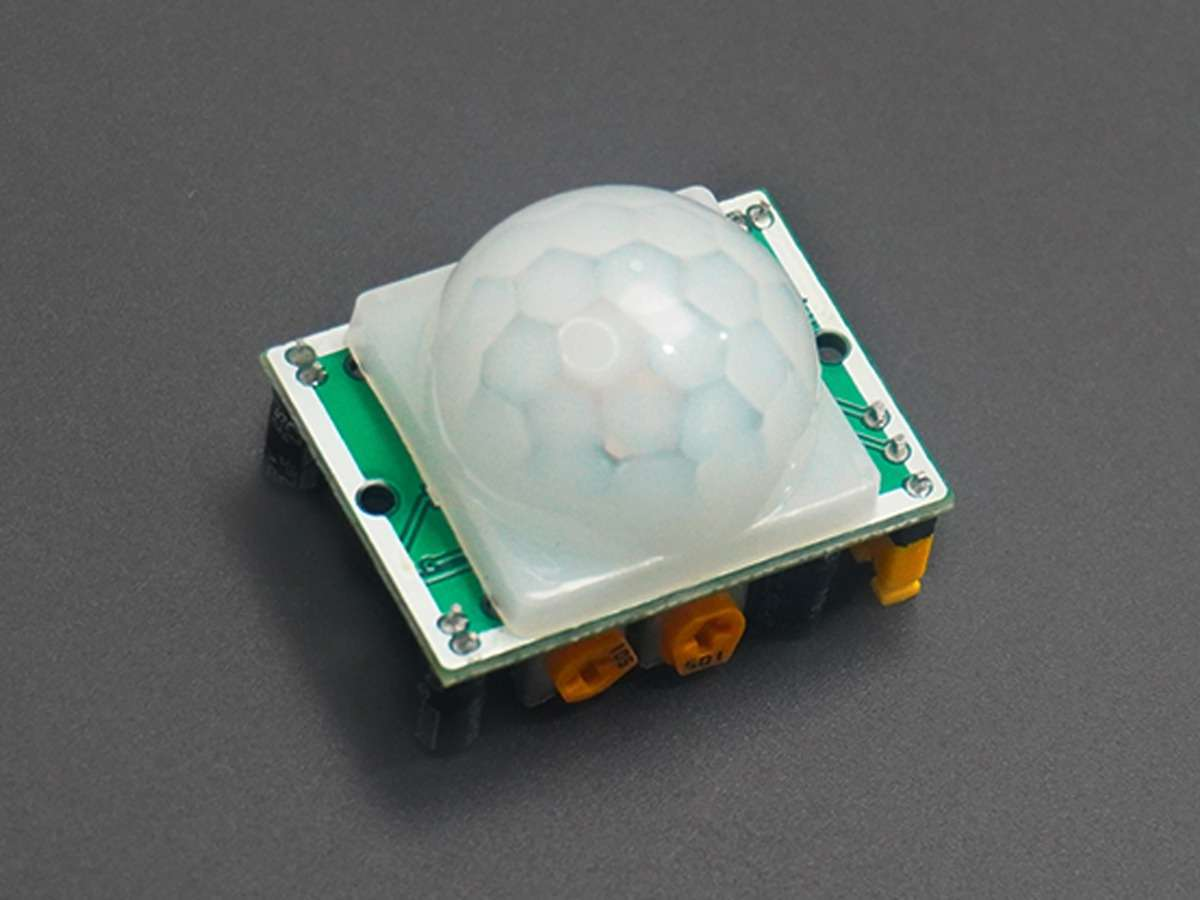
\includegraphics[width=0.48\textwidth]{Images/PIR.jpg}
%     \caption{Passive Infrared Sensor (PIR)}
%     \label{fig:PIR}
% \end{wrapfigure}

\paragraph{Passive Infrared Sensors}
Passive Infrared (PIR) sensors are widely used for presence detection. These sensors detect changes in infrared radiation within their field of view, emitted by warm objects like humans. The PIR sensor consists of a pyroelectric sensor that generates voltage when detecting temperature changes, aided by a Fresnel lens that focuses the infrared radiation onto the sensor. The generation of a voltage is not enough to determine the position of objects in the environment, but the sensor has some other advantages. As passive devices, PIR sensors do not emit radiation, making them energy-efficient and non-intrusive. The sensor could be effective in detecting precense to determine whether or not to run inference on an image. However, using PIR sensors for this purpose might biased results, potentially increasing the detection counts near the edges of the frame. PIR sensors are typically used for automated lights. A PIR sensor is diplayed in Figure \ref{fig:PIR}.

\begin{figure}[H]    
    \centering
    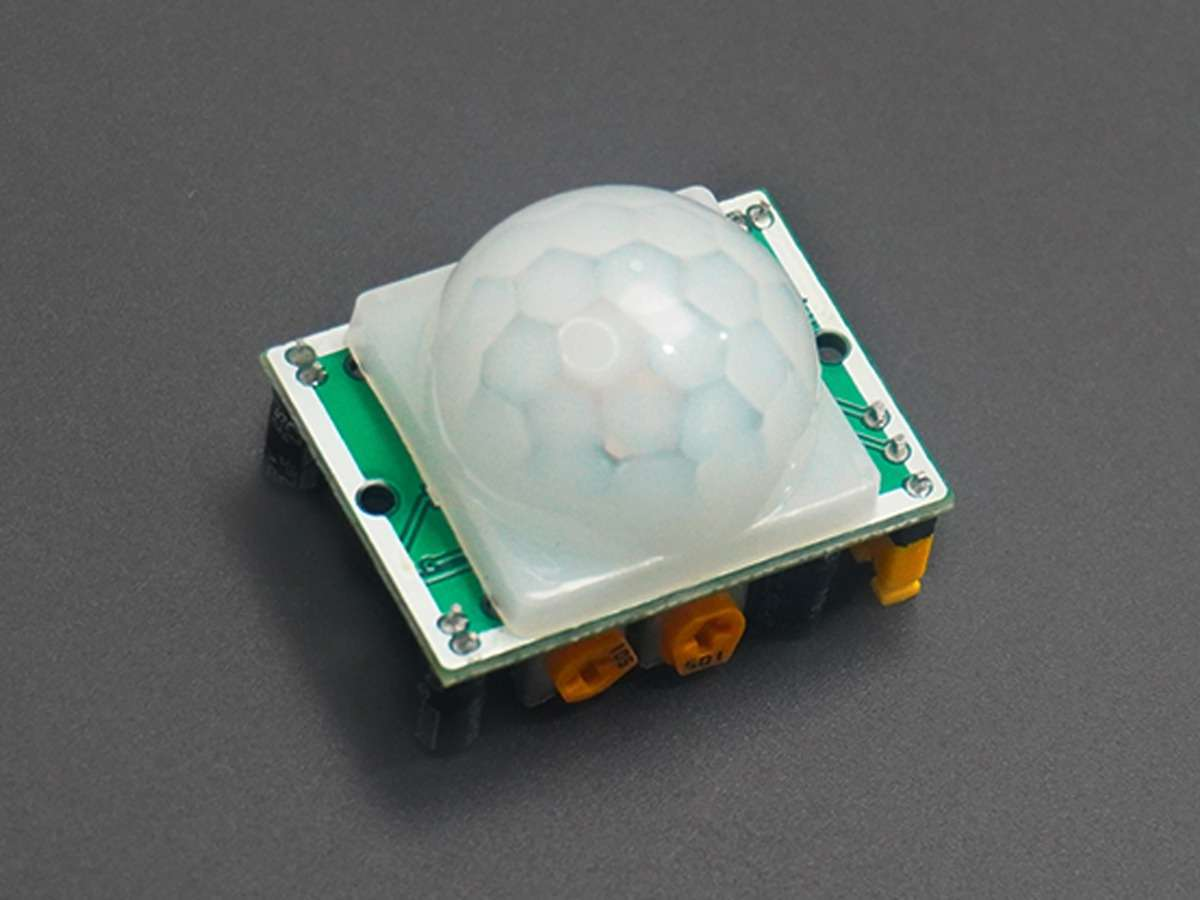
\includegraphics[width=0.4\textwidth]{Images/PIR.jpg}
    \caption{Passive Infrared Sensor (PIR)}
    \label{fig:PIR}
\end{figure}

\paragraph{Night Vision Cameras}
Night vision cameras are useful in low-light environments where traditional cameras falter. Most night vision cameras use passive infrared sensors to detect IR radiation naturally emitted by objects without actively illuminating them. However, some systems do include an IR illuminator that emits light to enhance the camera's ability to see in total darkness. Infrared imaging plays a crucial role in night-time pedestrian detection, forest fire detection, and maritime rescue. The capability to see in the low light conditions is particularly useful in settings like museums and aquariums, which often feature dim lighting to preserve exhibits or create atmospheric conditions. 

There are some challenges, however. The main issue with using IR images for machine learning is that they provide different information compared to visible-light images, which might affect the training and performance of models not adapted for IR data. Additionally, these cameras are typically more expensive and require more power compared to regular cameras due to the added components like IR illuminators. This which may limit their practicality for some applications. Furthermore, their effectiveness can be compromised by any obstructions that block IR light, such as windows or thick glasses. This makes them less preferable in aquariums filled with fish tanks. 

\paragraph{Radio Frequency Identification}
Radio Frequency Identification (RFID) is highly effective in medical and museum settings for tracking objects and people. This was seen in a study discussed in Section \ref{sec:visitor_behaviuor_analysis}, where RFID was used to track museum visitor movements through a museum. RFID technology can have a range of 3-4 meters(\cite{he2020medicalRFID}) which is sufficient for many indoor applications. Unfortuneately, they require wearable devices for tracking, which is a significant drawback for non-intrusive tracking. RFID's potential extends to applications like automatic medication adherence systems (see Figure \ref{fig:RFID_swallow}), which could reduce the workload on healthcare staff by ensuring patients take their medications without direct supervision.

\begin{figure}[H]    
    \centering
    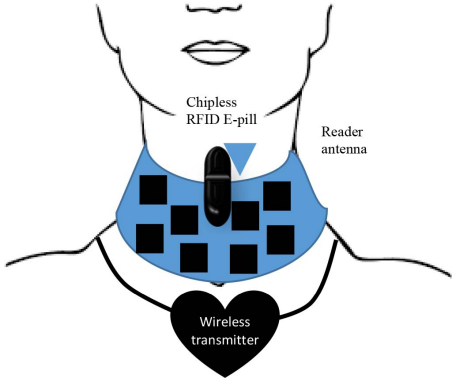
\includegraphics[width=0.5\textwidth]{Images/RFIDswallow.png}
    \caption{Proposed Design of a Pill System (\cite{he2020medicalRFID})}
    \label{fig:RFID_swallow}
\end{figure}

\paragraph{Sensors for Complex Environments}
In environments with obstacles that might block the line of sight, sound navigation and ranging (SONAR) can be particularly useful. SONAR sensors emit high-frequency sound waves (ultrasonic)\footnote{SONAR may also emit low-frequency sound waves, which is necessary in water but unlikely to be useful in an indoor application.} and detect their reflections to determine the changes in the environment and thus infer the presence of people. In \citeyear{ta2009sonarbasedhumanpresence}, \citeauthor{ta2009sonarbasedhumanpresence} proved human presence could be sensed with SONAR (ultrasonic) technology that was already present in most laptops in 2009. Further, it is worth mentioning that technologies like pressure sensors or systems detecting devices with Bluetooth or WiFi can also complement the presence detection/positioning in complex environments.
